% ACM TQC review manuscript: motivation, model, methods, results, and implications.
% Detailed protocols and complete control comparisons are in appendix.tex.
\PassOptionsToPackage{expansion=false}{microtype}
\documentclass[manuscript,screen,review,anonymous]{acmart}

\usepackage{amsmath,amssymb,amsfonts}
\usepackage{booktabs}
\usepackage{array}
\usepackage{graphicx}
\usepackage{placeins}
\usepackage{needspace}
% Allow small spacing adjustments before extending a line into the margin.
\setlength{\emergencystretch}{2em}

\setcopyright{none}
\acmJournal{TQC}
\acmYear{2026}
\acmDOI{}
% Publication volume, issue, and DOI are not assigned at submission.
\acmVolume{--}
\acmNumber{--}
\acmMonth{0}
\settopmatter{printacmref=true}

\begin{document}
\title[Channel Information beyond Aggregate QBER]{Beyond Aggregate QBER in Gate-Based BB84: Noise-Scaling Diagnostics and Basis-Aware Reconciliation}

% Author metadata is omitted in this repository edition.
\begin{abstract}
Whether disclosed BB84 observations identify a residual disturbance depends
on the implemented circuit and the assumed noise intervention. For depolarizing
gate noise with independently unknown Alice and Bob strengths, we formalize this
dependence through an observation map. Full operating transitions identify the
residual in PRIMARY and Scheme A; balanced B+ is nonidentifying at one setting,
but four distinct noise scales suffice to identify its polynomial intercept.
Unknown unscaled readout preserves identification of a combined residual while
confounding interception. Budget-matched likelihood comparisons separate these
structural statements from finite-sample precision. Across 81 conditions spanning
2000--32000 signals, three device pairs, and 2--20\% interception, full observations
have lower observed error in all 27 PRIMARY comparisons. Scheme A favors scaling
in 25 of 27 comparisons, with two reversals under weak interception; Monte Carlo
intervals quantify uncertainty in each accuracy difference. Profile likelihood
also separates residual precision from broad device uncertainty. A supporting
reconciliation study shows how finite-sample estimation can preserve or erase
conditional-information benefits, with long-block gains dominated by rate policies.
The contribution is a circuit-dependent classification of identifying observations,
tested precision tradeoffs, and explicit acquisition assumptions. Neither residual
disturbance nor reconciliation yield is a secure-key rate.
\end{abstract}

\begin{CCSXML}
<ccs2012>
 <concept><concept_id>10010583.10010786.10010813.10011726.10011727</concept_id><concept_desc>Hardware~Quantum communication and cryptography</concept_desc><concept_significance>500</concept_significance></concept>
 <concept><concept_id>10002978.10002979.10002980</concept_id><concept_desc>Security and privacy~Key management</concept_desc><concept_significance>300</concept_significance></concept>
 <concept><concept_id>10003033.10003083.10003014.10003015</concept_id><concept_desc>Networks~Security protocols</concept_desc><concept_significance>300</concept_significance></concept>
</ccs2012>
\end{CCSXML}
\ccsdesc[500]{Hardware~Quantum communication and cryptography}
\ccsdesc[300]{Security and privacy~Key management}
\ccsdesc[300]{Networks~Security protocols}
\keywords{BB84, quantum key distribution, information reconciliation, basis-aware decoding, LDPC, zero-noise extrapolation, noise diagnostics}

\maketitle
\raggedbottom

% Organize the contribution around channel observations, information targets, and costs.
\section{Introduction}
The implemented circuit determines what a BB84 diagnostic can learn from
already disclosed observations. Some paths expose a residual disturbance directly;
others allow it to be separated from device noise only by combining several
conditional rates. A balanced implementation can remove that contrast entirely.
Aggregate quantum bit error rate (QBER) hides these distinctions, but merely
retaining more labels does not guarantee that the target becomes identifiable.
The physical observation map must be examined first.

This leads to three questions. Which observations identify the target? When does
acquiring additional observations improve its precision? When does estimating
available channel structure improve recovery? The first is a structural question
about a specified model. The second concerns finite data and the cost of a noise
intervention. The third concerns the errors at the actual operating setting,
where an estimated reliability contrast can improve decoding or cause harm.

Gate-based BB84 makes these questions concrete. Complete preparation and receiver
paths determine how each bit encounters noise. A diagnostic acquisition discloses
all sifted bits, so Alice's bit, Bob's outcome, and the basis can all be retained.
A reconciliation frame instead discloses only a sample; its decoder may use Bob's
retained bits and public bases, but not Alice's undisclosed word. Noise scaling
provides a further observation design by changing specified legitimate-device
operations and acquiring fresh signals. These different information sets and
budgets share a conditional-channel model but serve distinct tasks.

Our central result is a circuit-dependent identification statement. Under ideal
intercept-resend and the declared depolarizing law, full operating transitions
identify the residual with unequal, unknown device noise in PRIMARY and Scheme A.
Balanced B+ provides a negative control: its operating map is nonidentifying,
whereas four distinct exact scaling settings suffice to recover the residual
intercept. Unknown unscaled readout leaves a combined residual identifiable but
prevents attribution to interception alone. The result classifies what the
observations determine before an estimator is selected.

The experiments then distinguish identification from precision. Matched-range
designs compare scaling with basis observations and paid calibration. Full-data
comparisons span multiple circuits, budgets, interception fractions, and device
pairs. Their ordering depends on the operating condition, particularly under weak
interception in Scheme A. Profile likelihood further shows that uncertain device
parameters can coexist with useful residual precision. A supporting reconciliation
study connects the same information question to estimation, disclosure, and recovery
costs; it establishes a finite-sample mechanism rather than a competitive coding advance.

The paper makes three linked contributions.
\begin{enumerate}
\item \textbf{Circuit-dependent identification with an explicit scope.}
An observation map, parameter domain, and proposition distinguish operating-data
identification, nonidentification, sufficient scaling observations, and readout confounding.
\item \textbf{Precision comparisons under declared acquisition costs.}
Matched ranges and a budget/interception grid quantify accuracy differences between
observation designs, while target profiles separate residual and nuisance uncertainty.
\item \textbf{Finite-sample recovery evidence.}
Complete-path controls, frozen pooling rules, confirmation, and transfer identify
conditional benefits and harms, separating fixed-code effects from rate-policy outcomes.
\end{enumerate}
Conditional entropy, soft decoding, pooling, likelihood profiling, and extrapolation
are established tools. The advance is the identification classification and its
controlled precision comparison for these BB84 implementations, together with the
measured costs of learning conditional reliability. The studies do not implement
a joint diagnostic-and-decoding procedure.

Section~\ref{sec:setting} defines resources and prior work, and
Section~\ref{sec:mechanism} establishes the physical channel and information benchmarks.
Sections~\ref{sec:diagnostics} and~\ref{sec:precision} answer the identification and
precision questions; Sections~\ref{sec:methods}--\ref{sec:results} address recovery.
Section~\ref{sec:discussion} draws their implications and limits together.

% Define the information budget and outcome before discussing related methods.
\section{Setting and Related Work}
\label{sec:setting}
\subsection{Observations, outcomes, and resource budgets}
We consider BB84~\cite{bennett1984} with uniformly random bits and bases, independent
single-qubit signals, and an authenticated noiseless classical channel. Alice's bit is
$A$, Bob's measured bit is $B$, and the matching sifted basis is $Z\in\{\mathrm r,\mathrm d\}$.
Each reconciliation frame contains $n+S$ sifted bits: $S$ bits are disclosed for estimation
and $n$ are decoded. The circuit study uses $(n,S)=(1000,200)$; subsequent experiments
vary these sizes explicitly. Evaluation is conditional on the sifted length, without
modelling optical loss or a transmission rate. Appendix~\ref{app:inventory} maps the
cohorts to their resource budgets and outcomes.

Bob receives the basis labels, the disclosed sample, and a syndrome of Alice's retained
word under a parity-check matrix $H$ with $m$ rows. Subtracting his own syndrome yields
the syndrome of the error vector. Decoder inputs never include undisclosed Alice bits
or simulator error positions. Correctness is recorded using simulator truth only for
evaluation; independent 64-bit Toeplitz verification controls acceptance and any retry.

Reconciliation inputs are sampled from the exact per-path error probabilities under the
independent-shot model. The circuit probabilities follow the depolarizing expressions
below; physical controls use explicit density-state transitions, including dependence on
Alice's bit. This direct sampling reproduces the specified independent circuit statistics
without rerunning a quantum-state simulation for every bit. The binary-channel grid
separately varies its declared crossover probabilities and is not a circuit experiment.

For exact recovery indicator $I_{\mathrm{corr}}$, we report frame error rate (FER),
yield, and disclosure efficiencies:
\begin{align}
 \mathrm{FER}&=1-\mathbb E[I_{\mathrm{corr}}], &
 Y&=\frac{n-m-64}{n+S}I_{\mathrm{corr}},\label{eq:yield}\\
 f_{\mathrm{syn}}&=\frac{m}{n h_2(Q)}, &
 f_{\mathrm{EC}}&=\frac{m+64}{n h_2(Q)},\label{eq:efficiency}
\end{align}
where $h_2$ is binary entropy. We report the mean of $Y$, a reconciliation yield per
sifted bit before privacy amplification. It charges the sacrificed sample, every transmitted
syndrome row, and verification bits, including when rows are algebraically dependent.
Authentication costs are outside this metric. Aggregate circuit-study efficiencies use
the measured retained-block QBER; target QBER labels refer to generator expectations.

The separate diagnostic study counts every transmitted signal, including those discarded
by sifting. All its sifted bits are disclosed and produce no key. Its outcome is an estimate
of a model-defined residual disturbance, rather than frame recovery. Keeping these budgets
and targets distinct prevents a more accurate diagnostic estimate from being mistaken for
a reduction in the errors that reconciliation must correct.



\FloatBarrier
\subsection{Position relative to earlier work}
Low-density parity-check (LDPC) syndrome reconciliation and rate adaptation are established in
QKD~\cite{elkouss2009,elkouss2011,blind2012,martinez2013}. Mesiti et al.~\cite{mesiti2010}
combine quantum- and public-channel metrics in sparse-graph decoding; puncturing and
shortening also create position-dependent priors~\cite{blind2012}. Simultaneous basis and
information reconciliation~\cite{martinezmateo2024} uses protocol structure at a different
stage from the already-sifted frames studied here. Soft metrics for reverse reconciliation
in discrete-modulation continuous-variable QKD~\cite{origlia2026} concern a different
measurement channel. Our question is the finite-sample value of an already-public discrete
basis label, including the harm from estimating an unreliable contrast.

Practical reconciliation studies assess disclosure and recovery together
\cite{borisov2023,treeviriyanupab2024}. We follow that principle and add controls that
separate the prior, code, and selection policy. The irregular-code experiments use published
variable-degree profiles~\cite{elkouss2009}, but a different check construction; they test
transfer across constructions rather than reproduce a published optimized threshold.

Zero-noise extrapolation uses additional acquisitions to estimate an idealized observable
\cite{temme2017,li2017,giurgicatiron2020}, and its precision depends on the extrapolation
design~\cite{krebsbach2022}. Fiorini et al.~\cite{fiorini2024} already estimate interception density in noisy
BB84; their subsequent work uses the estimate for threshold-based detection
\cite{fiorini2026}. The distinction here is the observation design: full disclosed
transitions, basis averages, calibrated references, and aggregate scaling are
compared under explicit device assumptions and equal transmitted budgets.
Qi et al.~\cite{qi2007dualdet} instead alternate a quiet detector for bounding
Eve's information with a fast detector for key generation. Our observation-map
analysis asks which disclosed gate-path statistics identify a modeled residual
under unknown device noise; it supplies neither a detector-switching protocol
nor their security bound. We evaluate the published interception-density formula
on its native law and on the gate-response law, without claiming to reproduce
the full attack-detection framework. Abstract parameter scaling is not itself a
hardware implementation of digital folding.

Implementation security additionally requires source and detector assumptions, finite-key
parameter estimation, and privacy amplification
\cite{gllp2004,scarani2009,xu2020,fung2009,tomamichel2012,rennerkoenig2005}.
Neither $Y$ nor the diagnostic estimate is a secure-key rate. The computational contribution
is to characterize when implementation-specific information improves an engineering task
within those broader requirements.

% Complete paths include the receiver rotation and retained identity noise sites.
\section{Physical Channel Structure and Its Information Value}
\label{sec:mechanism}
\subsection{Receiver gates complete the exposure count}
Figure~\ref{fig:circuits} shows the actual preparation and matched-basis measurement paths.
PRIMARY prepares rectilinear zero without a gate, uses $X$ for rectilinear one, and uses $H$
or $XH$ for the diagonal states. Scheme~A adds an identity to every preparation, so every
path has nonzero exposure. Scheme~B uses two preparation gates for each state. Bob still
applies $H$ before diagonal measurement; B+ adds an identity before rectilinear measurement
to balance the complete paths. Each identity is retained as an explicit noise site.

% Identity operations are experimental noise carriers. Compiler removal would
% change the physical model; circuit exports retain all operations explicitly.
\begin{figure}[htbp]
\centering
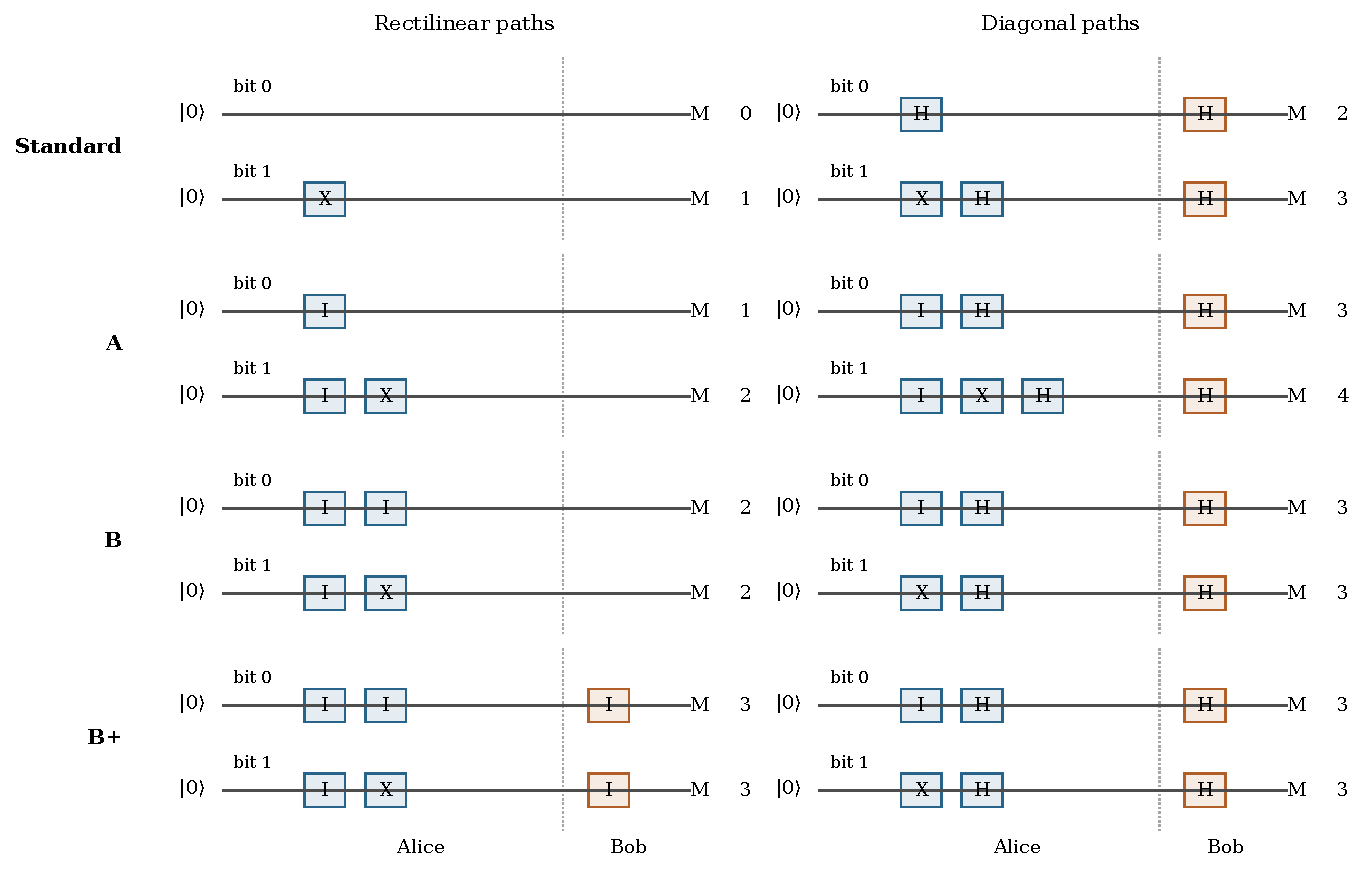
\includegraphics[width=0.96\linewidth]{images/complete_circuits.pdf}
\caption{Complete source circuits, with gates ordered from left to right. The dotted boundary separates Alice's preparation from Bob's measurement rotation; the number at right counts noisy gates. All paths start in $|0\rangle$, and the indicated bit determines the preparation. Orange gates belong to Bob. B+ adds a noisy identity on his rectilinear path. Measurement itself is noiseless.}
\Description{Four encodings, each with two bit paths in each basis. PRIMARY has complete counts 0/1 and 2/3; A has 1/2 and 3/4; B has 2/2 and 3/3; B+ has 3/3 and 3/3.}
\label{fig:circuits}
\end{figure}

For a homogeneous depolarizing channel
$\mathcal D_p(\rho)=(1-p)\rho+pI/2$ after each gate, covariance under ideal gates gives
\begin{equation}
 q_k(p)=\frac{1-(1-p)^k}{2}.
 \label{eq:gate}
\end{equation}
The complete gate counts for the two bit values are $(0,1;2,3)$ in PRIMARY,
$(1,2;3,4)$ in A, $(2,2;3,3)$ in B, and $(3,3;3,3)$ in B+, where the semicolon separates
rectilinear and diagonal bases. The basis error probability is the average over its two
bit paths. In B, the ratio is $q_3(p)/q_2(p)$; at 10\% total target QBER it is 1.437.
The additional receiver Hadamard explains the residual asymmetry. Exact density-matrix
checks verify all paths and the two-hop intercept-resend model used below.

Scheme~A is a mechanism control rather than a proposed encoding optimization. Its identities
remove a literal zero-noise path while preserving exposure differences. B+ supplies the
corresponding negative control for basis information. Together they separate the source
of the effect from the special bare-state path in PRIMARY.

\subsection{A basis-independent channel attenuates the signal}
We insert an independent depolarizing link between preparation and reception, with bit-error
probability $c$ in either basis. Isotropy allows this channel to be commuted to the end of
the path for calculation. The resulting basis probabilities are
\begin{equation}
 p_z^{\mathrm{tot}}=c+(1-2c)p_z^{\mathrm{gate}},\qquad z\in\{r,d\}.
 \label{eq:channel}
\end{equation}
At fixed total QBER $Q$, the average gate contribution is $(Q-c)/(1-2c)$. Increasing $c$
therefore reduces the basis contrast, reaching zero at $c=Q$. This control isolates noise
composition from an increase in overall decoding difficulty.

\subsection{From transition probabilities to useful information}
Write $W_f(b\mid a,z)$ for the channel from Alice's bit to Bob's measured bit,
conditional on the public basis and a specified noise scale $f$. Reconciliation
uses $W_1$; diagnostics probe how the channel changes with $f$. Under independent
uniform input bits and bases, the complete transition law determines the joint
probabilities $P(A=a,B=b,Z=z)=W_1(b\mid a,z)/4$.

For asymptotically reliable one-way reconciliation with known channel probabilities,
conditional entropy supplies the classical benchmark~\cite{slepian1973,elkouss2011}.
The information made available by retaining the basis is
\begin{equation}
 G=H(A\mid B)-H(A\mid B,Z)=I(A;Z\mid B)\geq0.
 \label{eq:information}
\end{equation}
For basis-conditioned binary symmetric channels (BSCs),
\begin{equation}
 H(A\mid B,Z)=\sum_z P(Z=z)h_2(p_z),\qquad
 G=h_2(Q)-\sum_z P(Z=z)h_2(p_z).
 \label{eq:mixtureentropy}
\end{equation}
These are established information identities, not predictions of finite-length BP
performance. The BSC reduction is inappropriate when error probabilities depend
on Alice's bit; then we compute both entropies from the full transition law.

There is also a distinction between knowing the basis and using the full channel.
For error bit $U=A\oplus B$, a basis-only Bernoulli prior has ideal expected
log loss $H(U\mid Z)$, whereas a transition-aware prior can attain
$H(U\mid B,Z)=H(A\mid B,Z)$. Their difference
$D_B=I(U;B\mid Z)$ measures the additional information in Bob's local bit after
conditioning on basis. It is distinct from $G$, whose comparator already uses $B$.
In an asymmetric channel, observing $B=0$ or $B=1$ can change the probability
that a position is erroneous even at fixed $Z$. Thus asymmetric readout can
have $D_B>0$ while $G=0$; thermal relaxation can provide both kinds of information.
These are population log-loss opportunities, not guaranteed finite-sample yield gains.
Neither quantity establishes what an eavesdropper learns.

% BEGIN GENERATED INFORMATION_TABLE
\begin{table}[!htbp]
\centering
\small\setlength{\tabcolsep}{4pt}
\caption{Channel information for the five B+ controls matched to $Q=6\%$. Values are bits per retained bit, computed from the stored transition probabilities with uniform input bits and bases. $G=I(A;Z\mid B)$ is the basis benefit relative to a decoder already using $B$; $D_B=I(U;B\mid Z)$ is the extra ideal error-prior log-loss reduction from Bob\textquotesingle s bit after conditioning on basis. These are distinct quantities and are not added together.}
\label{tab:information}
\begin{tabular}{@{}lrrrr@{}}
\toprule
Mechanism & $H(A\mid B)$ & $H(A\mid B,Z)$ & $G$ & $D_B$ \\
\midrule
Homogeneous & 0.32744 & 0.32744 & 0.00000 & 0.00000 \\
Gate-dependent & 0.32705 & 0.30538 & 0.02166 & 0.00088 \\
Pauli link & 0.32744 & 0.30977 & 0.01768 & 0.00000 \\
Thermal & 0.29886 & 0.29257 & 0.00629 & 0.03274 \\
Readout & 0.29758 & 0.29758 & 0.00000 & 0.02986 \\
\bottomrule
\end{tabular}
\end{table}
% END GENERATED INFORMATION_TABLE

The matched physical controls quantify why these distinctions matter
(Table~\ref{tab:information}). At the same 6\% QBER,
$G$ is 0.02166 bits per retained bit for gate-dependent noise and 0.01768 for the
Pauli link, but zero for homogeneous noise and asymmetric readout. Readout nevertheless
has $D_B=0.02986$: its useful structure is in the measured bit rather than the basis.
Thermal relaxation likewise has a larger local-bit increment than its basis benefit.
These population opportunities motivate the finite-sample comparisons in
Section~\ref{sec:results}. Identifying the origin of a disturbance additionally requires a specified
physical model and observations that identify its parameters. The next section
asks which parts of the disclosed channel and its noise response meet that need.

% Diagnostics acquire additional signals and have a different target from recovery.
\FloatBarrier
\section{Which Observations Identify the Residual?}
\label{sec:diagnostics}
\subsection{Physical assumptions and the residual target}
Table~\ref{tab:assumptions} distinguishes the assumptions used by each diagnostic comparison.
\begin{table}[!htbp]
\centering
\small\setlength{\tabcolsep}{4pt}
\caption{Diagnostic assumptions and targets. All rows assume the stated gate paths
and independent stationary signals. Characterizing the scaling intervention is
separate from fitting its unknown baseline noise strengths.}
\label{tab:assumptions}
\begin{tabular}{@{}>{\raggedright\arraybackslash}p{.19\linewidth}>{\raggedright\arraybackslash}p{.34\linewidth}>{\raggedright\arraybackslash}p{.42\linewidth}@{}}
\toprule
Case & Device and observation assumptions & Identified target and scope \\
\midrule
Basis/range study & Equal $p_A=p_B$; ideal Eve; no readout noise &
PRIMARY's two operating basis rates identify $e_0=r/4$. \\
Full-transition study & Independently unknown $p_A,p_B$; ideal Eve; no readout noise &
PRIMARY and A identify $e_0$ at one setting. B+ requires additional identifying observations. \\
Scaled B+ & Same unknown devices; four distinct admissible scales &
Aggregate rates identify $e_0$ by cubic interpolation; four is sufficient, not claimed minimal. \\
Unknown readout & A common unscaled symmetric flip $c$; ideal Eve &
Identifying observations recover $e_c$, not $r$ separately. Known $c<1/2$ allows inversion. \\
Noisy-Eve controls & Fixed known $p_E$ with legitimate devices scaled &
Target is $r q_I(0,0,p_E)$. The ideal-Eve proposition does not apply. \\
\bottomrule
\end{tabular}
\end{table}

Disturbance diagnostics probe the response of the channel to additional measurements.
Their meaning depends on which device operations the intervention changes. Eve independently intercepts fraction $r$, measures in a uniformly random
basis, and resends her result. Let $p_A,p_B,p_E$ denote per-operation depolarization
for Alice, Bob, and Eve. Scaling only legitimate devices gives
\begin{equation}
 Q_f=(1-r)q_0(fp_A,fp_B)+r q_I(fp_A,fp_B,p_E),\qquad
 e_0=\lim_{f\to 0} Q_f=r\,q_I(0,0,p_E).
 \label{eq:separatedresponse}
\end{equation}
Here $q_0$ and $q_I$ are the exact unintercepted and intercepted PRIMARY-path
probabilities (Appendix~\ref{app:diagnostic}). With ideal Eve, $e_0=r/4$.
Fixed noisy Eve generally changes this coefficient. Scaling Eve's operations as well
defines an all-scaled control, for which the limit again equals $r/4$.
The mathematical limit defines the target; acquisition settings need not include zero.

The general law allows $p_A\ne p_B$. The nominal comparisons impose $p_A=p_B=p$. A targeted held-out-setting experiment
also fits independently unknown legitimate-device parameters; fixed noisy-Eve
controls assume known $p_E$. Sifted and error
counts are sampled as $N\sim\mathrm{Binomial}(T,1/2)$ and
$E\mid N\sim\mathrm{Binomial}(N,Q_f)$, exactly representing independent shots
under the stated model. Density-state calculations independently check the response.

\subsection{Aggregation loses information already present in basis labels}
Under ideal Eve and equal legitimate-device noise, the response reduces to
\begin{equation}
 Q_f=\frac r4+\left(1-\frac r2\right)q_0(fp,fp).
 \label{eq:idealresponse}
\end{equation}
A single $Q_1$ leaves a continuum of admissible device-noise and interception pairs:
$r=[Q_1-q_0(p,p)]/[1/4-q_0(p,p)/2]$ wherever the parameters remain physical.
This is a structural ambiguity, not merely sampling uncertainty.

Figure~\ref{fig:ambiguity} gives an exact example from the response law. The nominal-grid
state $(p,r)=(0.015,0.10)$ and a noise-only state $(p,r)\simeq(0.049024,0)$ both
give $Q_1=3.5581\%$, yet their residuals are 2.5\% and zero. The states respond
differently when legitimate-device noise is scaled, but their basis-resolved QBERs
also differ at $f=1$: the rectilinear/diagonal pairs are $(2.8563\%,4.2600\%)$ and
$(1.2256\%,5.8906\%)$. Thus basis labels already distinguish these states without
a scaling intervention. The example establishes a loss from aggregation, not a
need for noise scaling.

Under the same ideal-Eve, equal-device-noise model, let $Q_r,Q_d$ be the population
basis rates at $f=1$. Then
\begin{equation}
 Q_z=\frac r4+\left(1-\frac r2\right)q_z(p),\qquad
 q_r(p)=\frac p4,\quad q_d(p)=\frac{5p-4p^2+p^3}{4}.
 \label{eq:basisdiagnostic}
\end{equation}
Writing $\eta=(Q_d-Q_r)/(1-2Q_r)$ gives $\eta=p-p^2/2$, hence
\begin{equation}
 p=1-\sqrt{1-2\eta},\qquad r=\frac{4Q_r-p}{1-p/2}.
 \label{eq:basisinverse}
\end{equation}
The inverse is unique for $0\leq p<1$ and $0\leq r\leq1$. A single basis-resolved
setting therefore identifies the two parameters in this model. Finite samples can
still make the inverse imprecise, undefined, or outside the physical domain;
Appendix~\ref{app:diagnostic} specifies how singular counts and invalid roots are handled.
The value of additional settings must be assessed against this existing information,
with the same signal budget, rather than against aggregate $Q_1$ alone.

\begin{figure}[!htbp]
\centering
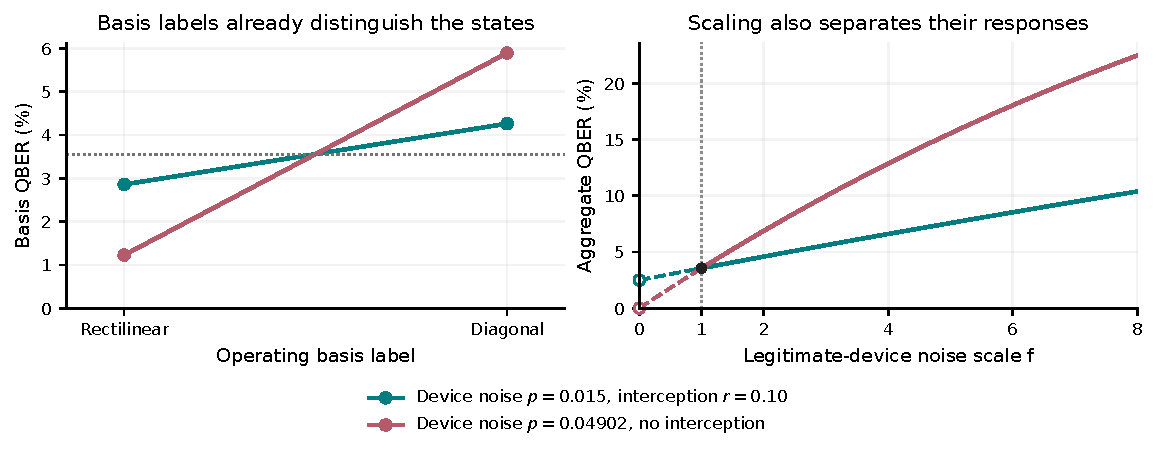
\includegraphics[width=0.97\linewidth]{images/aggregate_ambiguity.pdf}
\caption{Two ways to resolve an aggregate-QBER ambiguity in the ideal-Eve model.
Left: the same operating aggregate QBER, 3.5581\% (dotted line), conceals distinct
rectilinear and diagonal rates. Right: the states also have different scaling
responses and zero-noise limits. Basis labels alone already distinguish this pair.
These are exact model evaluations checked by density-state propagation; dashed
segments and open points denote the unmeasured extrapolation region and limits.}
\Description{The two states have different basis-specific rates despite equal
aggregate QBER. Their noise-scaling curves intersect at scale one but have residuals
of 2.5 percent and zero.}
\label{fig:ambiguity}
\end{figure}

\subsection{An observation map and identification result}
For ideal Eve, a path containing $k_A$ Alice gates and $k_B$ Bob gates has
\begin{equation}
 Q_{az}(f)=\frac12-\left(\frac12-\frac r4\right)
 (1-fp_A)^{k_A(a,z)}(1-fp_B)^{k_B(a,z)}.
 \label{eq:attack}
\end{equation}
Fix a known circuit $C$ and positive scales $F=\{f_1,\ldots,f_J\}$, with
$f_{\max}=\max(\{1\}\cup F)$. The domain is
$\Theta_F=\{(p_A,p_B,r):0\leq p_A,p_B<1/f_{\max},\;0\leq r\leq1\}$.
Let $\Phi_C(\theta)$ be the four operating probabilities in the order
$(0r,1r,0d,1d)$ and $\Psi_{C,F}(\theta)=(Q_{f_j})_{j=1}^J$ the aggregate
scaling probabilities. A target is identified by a map if equal map values
always imply equal target values. This is a population statement, separate
from the accuracy of an estimator based on finite counts.

\Needspace{18\baselineskip}
\begin{proposition}[Circuit-dependent residual identification]
\label{prop:identification}
Under Eq.~\eqref{eq:attack} on $\Theta_F$:
\begin{enumerate}
\item For PRIMARY and Scheme A, $\Phi_C$ identifies $(p_A,p_B,r)$ and hence
$e_0=r/4$. In PRIMARY the rectilinear-zero path directly measures the residual:
\begin{equation}
 \Pr(B\ne A\mid A=0,Z=\mathrm r)=e_0.
 \label{eq:subset}
\end{equation}
\item For B+, $\Phi_C$ does not identify $e_0$ on the domain; at interior
parameter points, the same operating observation admits a continuum of residuals. Four distinct admissible
scales suffice for $\Psi_{C,F}$ to identify $e_0$. This is a sufficiency result,
not a minimum-setting claim or a requirement to estimate every nuisance parameter.
\item If an unknown common symmetric readout flip $0\leq c<1/2$ is unscaled,
the identifying observations above instead identify
\begin{equation}
 e_c=c+(1-2c)r/4.
 \label{eq:residual}
\end{equation}
They do not generally identify $c$ and $r$ separately. If $c$ is known,
$r=4(e_c-c)/(1-2c)$.
\end{enumerate}
\end{proposition}
\begin{proof}
Write $u=1-p_A$, $v=1-p_B$, $d=1-r/2$, and $s_{az}=1-2Q_{az}(1)$.
The contraction vectors are $d(1,u,uv,u^2v)$ for PRIMARY and
$d(u,u^2,u^2v,u^3v)$ for A. Their entries are positive on the domain.
PRIMARY gives $d=s_{0r}$, $u=s_{1r}/d$, and $v=s_{0d}/(du)$;
A gives $u=s_{1r}/s_{0r}$, $d=s_{0r}/u$, and $v=s_{0d}/(du^2)$.
These determine all three parameters.

B+ has only $s=du^2v$ at one setting. Holding $p_B$ fixed while replacing $p_A$
by nearby $t$ and $r$ by $2[1-s/\{(1-t)^2(1-p_B)\}]$ preserves $s$ and
varies the residual within the interior domain. Across scales,
$Q_f=\{1-d(1-fp_A)^2(1-fp_B)\}/2$ is a polynomial of degree at most three.
Four distinct exact values determine its intercept, $Q_0=(1-d)/2=e_0$.
An unscaled readout flip replaces $d$ everywhere by $(1-2c)d$, preserving
the inverses and intercept argument for $e_c$. Different $(c,r)$ pairs can
have this same product, proving the attribution ambiguity.
\end{proof}

The same log-linear argument applies to other path counts: writing
$\log s_j=\log d+k_{A,j}\log u+k_{B,j}\log v$, a matrix with rows
$(1,k_{A,j},k_{B,j})$ of rank three identifies all three parameters on the
positive domain. Distinct monomials alone do not ensure that rank.
For scaling, three values do not determine a general cubic: adding
$\kappa\prod_{j=1}^3(f-f_j)$ preserves them while changing its intercept at
positive $f_j$. Whether restrictions on the physical coefficients permit fewer
settings requires a separate identification argument. Neither minimum setting
count nor numerical stability follows from parameter counting.

The proposition distinguishes preserving information from intervening on the
channel. The PRIMARY subset uses only an expected $T/8$ signals, while a full
likelihood can use the other disclosed strata too. Scheme A identifies the same
target without a gate-free path, but identification alone does not ensure equal
precision. B+ illustrates the need for observations beyond the operating map;
four scales provide one sufficient design under the assumed response law.

\subsection{Operational meaning of the scaling law}
The transformation $p_A\mapsto fp_A$, $p_B\mapsto fp_B$ is a characterized
intervention in the simulation. One model-level realization adds randomized
Pauli noise after each legitimate-device gate. Since
$\mathcal D_{\eta}\circ\mathcal D_p=\mathcal D_{p+\eta-p\eta}$, choosing
\begin{equation}
 \eta(f,p)=\frac{(f-1)p}{1-p},\qquad 1\leq f,\quad fp<1,
 \label{eq:injection}
\end{equation}
gives the required channel. The injected Pauli probabilities are $\eta/4$
for each of $X,Y,Z$ and $1-3\eta/4$ for identity. A hardware implementation
would need independently characterized baseline noise, calibrated injection,
and accounting for errors introduced by the injection operations themselves.

Gate folding and pulse stretching supply different physical controls
\cite{giurgicatiron2020,temme2017}. Under identical independent depolarization,
$k$ repeated noise applications give $1-(1-p)^k$, which agrees with $kp$ only
to first order. Stretching time in a stationary exponential decay has the same
nonlinear form. Large nominal factors therefore cannot be interpreted as the
linear law without calibrating the actual response and updating the model.
One must also check path dependence, readout stability, and stationarity across
settings; interleaving settings can separate acquisition order from a drift trend.
Time-correlated noise can change its spectral response under amplification
\cite{schultz2022}. Other possible hardware departures include changing crosstalk
during stretched pulses, gate-dependent leakage, and control-pulse distortion.
These could introduce scale-dependent systematic errors outside the assumed
polynomial response. More shots would reduce sampling error without removing
that bias; response checks and an appropriate hardware model would be needed.
These mechanisms are not simulated here.

Our comparisons condition on a known scale map and charge transmitted signals
$T$. They do not include control-characterization cost, extra gate duration, or
uncertainty in the calibrated scale. Absence of a paid Eve-free reference in a
scaling acquisition does not mean absence of device calibration. Hardware
precision or cost advantages require these additional resources to be assessed.
If characterization also determines $p_A,p_B$, that information must be supplied
to the operating-data comparator; it changes the unknown-device problem studied here.

% Precision comparisons condition on an identified target and a declared observation design.
\section{When Do Additional Acquisitions Improve Precision?}
\label{sec:precision}
\subsection{Compare acquisition strategies under the same budget}
The range comparison uses a single basis-resolved operating acquisition,
two- or four-setting aggregate scaling, and calibrated inversion. Each pays the
same transmitted budget $T$; calibration assigns 30\% to an independent Eve-free
reference and 70\% to the attacked setting. The nominal 48-cell grid crosses
$p\in\{0.005,0.015,0.03,0.06\}$, $r\in\{0,0.1,0.2,0.4\}$, and
$T\in\{2000,8000,32000\}$, with 500 replicates per cell. Nine interior cells
at $T=8000$ provide interpolation validation without retuning.

Both setting counts use scaling caps 2.5, 4, and 8. A finite minimax Fisher search
selects locations and positive allocations before sampling. Weighted least squares
(WLS) uses Jeffreys plug-in variances and signed interception estimates; observed
coverage evaluates its local-Wald intervals. The direct basis inverse reuses the
basis counts without parameter projection. Other acquisitions are independent.
Appendix~\ref{app:range} specifies designs, bounds, calibration inversion, and
every numerical comparison (Table~\ref{tab:validation}).

\subsection{Basis resolution is a strong baseline; scaling depends on its range}
Figure~\ref{fig:diagnostics} summarizes the budget-matched range comparison.
On the nominal grid, the single-setting basis fit has mean absolute error (MAE)
0.504 pp, compared with 0.516 pp for two-setting scaling up to $f=8$ and
0.552 pp for calibrated inversion. Thus the basis label can support accurate
residual estimation in this model without either a reference acquisition or a
noise-scaling intervention. The result concerns the specified physical model and
estimator, not a general replacement for calibration.



\begin{figure}[!htbp]
\centering
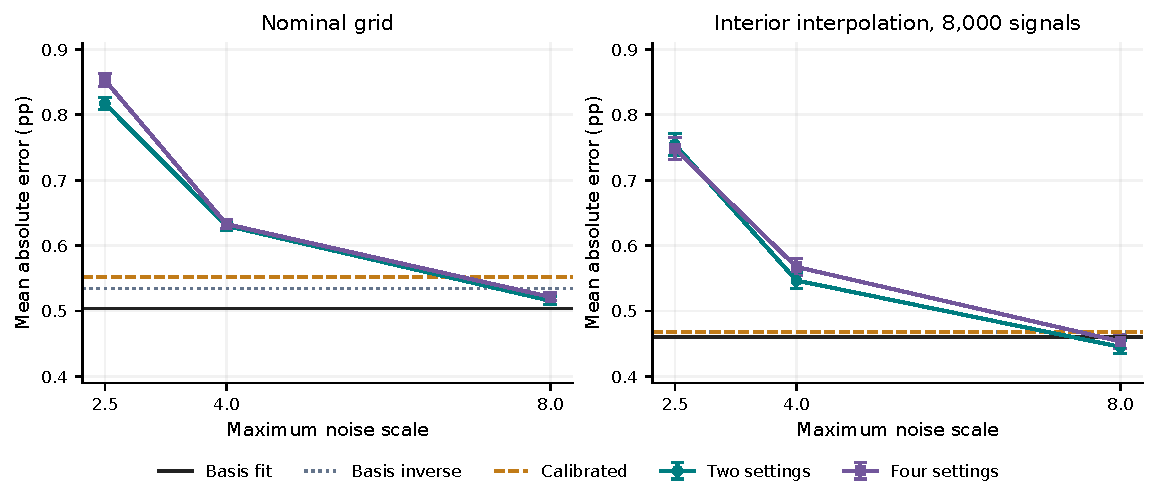
\includegraphics[width=0.97\linewidth]{images/diagnostic_comparison.pdf}
\caption{Matched-range diagnostic comparisons. Left: equal-cell mean MAE over the
48 nominal cells; right: the nine interior interpolation cells at 8000 signals. Two- and
four-setting designs are selected before sampling from the same bounded range.
Horizontal lines show the single-setting basis estimators and calibrated inversion.
Error bars are 95\% Monte Carlo intervals conditional on each fixed grid; they do
not include deployment or design-selection uncertainty.}
\Description{Increasing the maximum scaling factor reduces error for both aggregate
designs. At restricted ranges they exceed the basis baseline; at scale eight the
ordering depends on the grid and the basis estimator.}
\label{fig:diagnostics}
\end{figure}

Figure~\ref{fig:diagnostics} shows that range has the larger effect. Restricting
two-setting scaling to $f_{\max}=2.5$ or 4 raises nominal MAE to 0.817 or
0.630 pp. Four-setting fits at the same limits give 0.853 and 0.633 pp, and
reach 0.521 pp at $f_{\max}=8$. The large improvement over the reference
cohort's equally allocated, narrow-range four-setting fit therefore should not be
attributed to the number of settings alone.

On the interior interpolation cells, two-setting scaling at $f_{\max}=8$ gives 0.445 pp versus
0.461 pp for the basis fit: a difference of -0.016 pp with Monte Carlo 95\%
interval [-0.030,-0.001]. The nominal ordering also changes when the unrestricted
basis inverse replaces the constrained fit: its MAE is 0.534 pp. These small
comparisons support a conditional choice of acquisition and estimator, rather
than uniform superiority or statistical equivalence. These range comparisons hold the observation reduction fixed. The full-data
comparison below tests how much the basis reduction itself discards.

Coverage is reported per cell with Wilson Monte Carlo intervals. For example,
450 covered intervals out of 500 gives 90\% coverage with interval
[87.1\%,92.3\%], so a threshold at 90\% is not a sharp classification of
reliability. Grid averages in Table~\ref{tab:validation} summarize the design;
the complete cell-level errors, coverage intervals, and boundary fits accompany
the data.

\FloatBarrier
\subsection{Full disclosed data and cross-circuit validation}
The cross-circuit comparison uses 8000 signals and 500 replicates in each of
three device pairs, with $r=0.2$. The operating acquisition records all four
bit-and-basis strata; subset, basis-average, and full estimators reuse it.
An independent scaling acquisition uses the previously fixed cap-4 design
$f=(1,3,3.5,4)$ with shares $(0.70,0.05,0.05,0.20)$ in every circuit.
It is transferred unchanged, not optimized separately for each circuit.
All likelihood fits use physical bounds $p_A,p_B\in[0,0.24975]$, $r\in[0,1]$.
Full-transition and scaling fits estimate the two devices independently; the
basis-only fit imposes equal noise. Subset intervals are Wilson intervals~\cite{wilson1927};
likelihood fits profile nuisance parameters for nominal 95\% residual intervals.
Empirical coverage is measured because boundaries can invalidate the usual
asymptotic calibration~\cite{fischer2021}.

% BEGIN GENERATED CROSS_CIRCUIT_TABLE
\begin{table}[!htbp]
\centering
\small\setlength{\tabcolsep}{4pt}
\caption{Cross-circuit diagnostics: 8000 transmitted signals, $r=0.2$, and 500 replicates per cell. Entries are residual MAE in percentage points (pp) / interval coverage (\%). The first three estimators share one operating acquisition; scaling uses an independent, equally budgeted four-setting acquisition. Basis assumes equal device noise; full and scaling fit the devices independently. \textit{Set} denotes nonidentification, so no point-estimator MAE is reported. Subset applies only to PRIMARY. Coverage has Monte Carlo uncertainty; cell-level intervals accompany the records.}
\label{tab:crosscircuit}
\begin{tabular}{@{}llllll@{}}
\toprule
Circuit & $(p_A,p_B)$ & Subset & Basis & Full & Scaling \\
\midrule
PRIMARY & $(.03,.03)$ & 0.552 / 95.6 & 0.552 / 95.2 & 0.504 / 94.6 & 0.588 / 96.6 \\
PRIMARY & $(.01,.05)$ & 0.532 / 95.6 & 0.666 / 90.2 & 0.444 / 95.8 & 0.575 / 95.6 \\
PRIMARY & $(.05,.01)$ & 0.523 / 95.2 & 0.656 / 90.0 & 0.488 / 95.8 & 0.628 / 98.0 \\
A & $(.03,.03)$ & -- & 1.020 / 93.8 & 1.114 / 96.6 & 0.708 / 96.8 \\
A & $(.01,.05)$ & -- & 1.488 / 77.0 & 0.809 / 97.4 & 0.600 / 96.2 \\
A & $(.05,.01)$ & -- & 1.515 / 83.8 & 1.182 / 94.2 & 0.862 / 98.0 \\
B+ & $(.03,.03)$ & -- & set / 100 & set / 100 & 0.738 / 96.6 \\
B+ & $(.01,.05)$ & -- & set / 100 & set / 100 & 0.676 / 97.0 \\
B+ & $(.05,.01)$ & -- & set / 100 & set / 100 & 0.849 / 96.6 \\
\bottomrule
\end{tabular}
\end{table}
% END GENERATED CROSS_CIRCUIT_TABLE

Table~\ref{tab:crosscircuit} shows how the circuit changes the baseline comparison.
In PRIMARY, retaining Alice's bit avoids the equal-device assumption and improves
precision over the subset in these three cells. Full-transition MAEs are
0.444--0.504 pp, with 94.6--95.8\% interval coverage, while four-setting aggregate
scaling gives 0.575--0.628 pp. In Scheme A the full-data estimator remains
identifiable but becomes less precise: at equal noise its MAE is 1.114 pp,
versus 0.708 pp for scaling. B+ has no identified single-setting point estimate;
the displayed operating intervals include a continuum of residuals. Its scaled
MAEs are 0.676--0.849 pp with 96.6--97.0\% coverage. Preserving all observations
is therefore the appropriate comparison; its advantage depends on the circuit.


\FloatBarrier
\subsection{Budgets and weak interception change the precision tradeoff}
\label{sec:precisiongrid}
The precision grid independently crosses all three circuits, the three device
pairs in Table~\ref{tab:crosscircuit}, $T\in\{2000,8000,32000\}$, and
$r\in\{0.02,0.10,0.20\}$. Each of 81 cells has 500 fresh replicate blocks,
including new acquisitions at the anchor conditions. Full-transition and aggregate
scaling strategies each receive their complete budget. The cap-4 locations,
allocations, likelihood, bounds, and profile construction remain fixed.
No parameter or design is selected using these outcomes. The study contains
40,500 blocks and 81,000 independently budgeted acquisitions.

For the 54 identified PRIMARY/A comparisons, define
$\Delta_{\rm MAE}=\mathrm{MAE}_{\rm full}-\mathrm{MAE}_{\rm scaling}$;
positive values favor scaling. We report pointwise 95\% Monte Carlo intervals
using the independent absolute-error variances and Welch critical values, together
with Bonferroni intervals covering all 54 comparisons simultaneously at nominal
95\%. These approximate intervals quantify simulation precision within the fixed
design, not deployment uncertainty or equivalence. B+ has no operating point
estimator for this contrast; its scaled outcomes are reported separately.

\begin{figure}[!htbp]
\centering
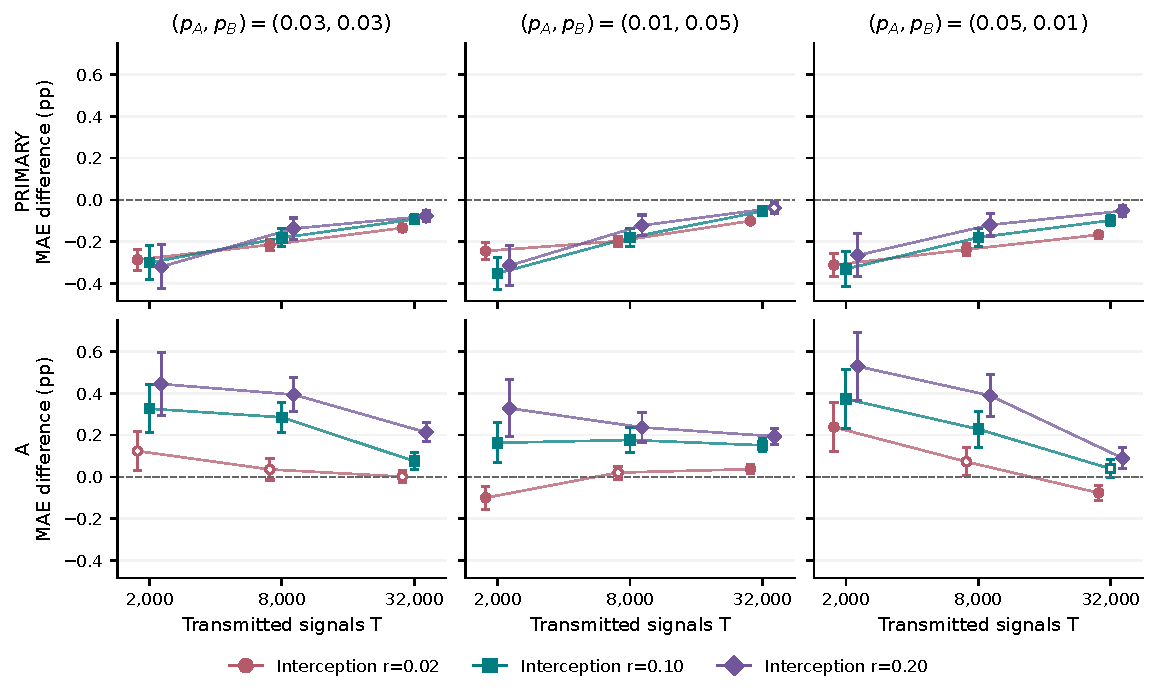
\includegraphics[width=.98\linewidth]{images/precision_grid.pdf}
\caption{Full-data minus scaling MAE across budgets and interception fractions.
Rows are PRIMARY and A; columns give device pairs. Positive values favor scaling.
Bars are pointwise 95\% Monte Carlo intervals from 500 independent acquisitions
per method and cell. Filled markers also exclude zero under simultaneous 95\%
Bonferroni intervals across all 54 comparisons; open markers do not. The fixed
scale design is transferred without retuning.}
\Description{Six panels show accuracy differences at three budgets for interception
fractions 0.02, 0.10, and 0.20. All PRIMARY differences favor full observations.
Scheme A mostly favors scaling, but two weak-interception cells favor full data.}
\label{fig:precisiongrid}
\end{figure}

PRIMARY has lower full-data MAE in all 27 point comparisons; 26 simultaneous
intervals exclude zero in that direction. Differences range from -0.352 to
-0.038 pp. Scheme A favors scaling in 25 of 27 point comparisons, with 19
simultaneous intervals supporting scaling and two supporting full data. Both
reversals occur at $r=0.02$: $T=2000$ with $(p_A,p_B)=(0.01,0.05)$ gives
$\Delta_{\rm MAE}=-0.100$ pp (pointwise interval [-0.154,-0.046]), and
$T=32000$ with $(0.05,0.01)$ gives -0.077 pp ([-0.114,-0.039]).
Thus the Scheme A ordering at $r=0.2$ does not extend uniformly to weak interception.

These are errors of the specified physically constrained estimators. In the
first reversed cell, the full/scaling target estimates reach zero in 38.4\%/29.4\%
of replicates; their biases are +0.082/+0.262 pp. This boundary behavior helps
describe why an accuracy ranking must accompany the identification result,
without attributing the reversal to a single cause. B+ scaling has empirical
profile coverage 94.8--99.6\% across its 27 cells. At $r=0.02,T=2000$, however,
its median interval widths are 3.20--4.15 pp for a residual of only 0.50 pp.
Coverage therefore coexists with limited resolution of weak disturbance; no
practical detection criterion is evaluated. Appendix~\ref{app:precisiongrid} gives every MAE contrast and the B+ uncertainty
summaries; all methods' coverage, bias, widths, and boundaries accompany the records.
The grid maps a within-model tradeoff; it does not
establish an optimal acquisition or robustness to an uncalibrated intervention.

\subsection{Held-out prediction exposes the limits of model checks}
A separate validation uses 8000 fitting signals and 2000 fresh signals at $f=2.3$,
which is absent from every fitted design. The total cost is therefore 10,000
signals per strategy. Five scenarios cover equal noise, an interior interpolation condition,
unequal Alice/Bob noise in both directions, and curvature that preserves the
operating point and zero-noise limit. The two- and four-setting designs are capped
at 4. Predictions include both fitted-parameter uncertainty and held-out sampling
uncertainty; validation counts never enter a fit.

The nominal equal-noise fits give held-out prediction coverage near 95\%, but a
prediction check need not detect a misleading residual estimate. With
$(p_A,p_B,r)=(0.01,0.05,0.2)$, the basis estimator's residual-interval coverage
falls to 87.8\%, while its held-out prediction coverage remains 92.8\%.
A response can be predicted reasonably at one extra setting even when the imposed
parameter relationship distorts the extrapolated target.

The same four-setting records also allow the device-equality assumption to be
relaxed. Signed weighted-least-squares fits yield very broad local-Wald intervals
and many device-boundary estimates (Table~\ref{tab:holdout}). Those outcomes
characterize that fitting procedure; they cannot establish that the target is
uninformative under every use of the observations.

\subsection{Target uncertainty differs from device uncertainty}
Weak identification of device noise need not imply weak identification of the
residual. We refit the five retained four-setting cohorts with binomial likelihood
and profile $e_0$, $p_A$, and $p_B$ separately. The residual intervals have median
widths 2.81--3.40 pp and 95.4--96.6\% coverage, compared with median widths
15.40--17.80 pp and upper-quantile widths above 200 pp for the signed-WLS Wald
intervals. Device intervals remain broad: median widths are 5.20--7.34 pp for
$p_A$ and 9.76--13.44 pp for $p_B$, against generating noise probabilities of
1--5\%. The likelihood information matrices are poorly conditioned, and about
half the noise estimates reach a boundary (Appendix~\ref{app:profiles}).
The boundary hits occur at zero nuisance noise; none of these 2500 fitted
interception fractions reaches its boundary, and no residual interval ends at
0 or $1/4$. The reported widths are therefore not set by clipping at the target
limits. Nevertheless, physical nuisance constraints restrict the profile search
and can affect its width. Coverage supports the procedure within these tested
conditions; it does not establish insensitivity to the bounds. Appendix~\ref{app:profiles}
details the boundary audit. The comparison also changes the fitting loss and
bounds, so the width difference cannot be attributed solely to profiling.

\subsection{Unscaled noise and drift change the target}
The readout-confounding statement in Proposition~\ref{prop:identification}
has a measurable consequence. At $c=1\%$, PRIMARY's full-data intervals cover
$e_c$ in 93.8--94.8\% of replicates across the three device pairs, but cover
the Eve-only value $r/4$ in only 74.2--74.6\%. Thus even full transitions and
scaling cannot separate $c$ and $r$ without additional information. A known
readout response or an appropriate Eve-free reference is needed for attribution.

The reference-and-stress cohort further tests calibration offsets, scaling
curvature, fixed noisy Eve, unscaled receiver noise, and time variation
(Appendix~\ref{app:diagnostic}). Unscaled noise changes the residual being
estimated; an attack ramp removes a single stationary target. These controls
delimit the model-based diagnosis rather than establish a universal estimator ranking.

% Estimator training, evaluation cohorts, and uncertainty are specified separately.
\section{Reconciliation Mechanism: Estimation and Experimental Design}
\label{sec:methods}
The diagnostic study concerns what observations identify about disturbance. We
now turn to predicting errors at $f=1$ well enough to improve
reconciliation. This evaluation uses a disclosed sample at that operating setting,
with no diagnostic acquisition or residual estimate supplied to the decoder.

\subsection{A shared centre and a sample-only pooling rule}
Let $E_z$ errors be observed among $S_z$ disclosed bits in basis $z$, with
$E=E_r+E_d$ and $S=S_r+S_d$. Define
\begin{equation}
 \widehat p=\frac{E+1/2}{S+1},\qquad
 \widetilde p=\frac ES,\qquad
 \widetilde p_z=\frac{E_z}{S_z}.
 \label{eq:pool}
\end{equation}
Separate Jeffreys estimates introduce a total of one pseudo-error across two classes,
whereas the pooled estimate introduces one half. To avoid crediting extra smoothing to
basis information, our main family retains one common centre:
\begin{equation}
 \widehat p_z(\lambda)=\widehat p+\lambda(\widetilde p_z-\widetilde p),
 \qquad 0\leq\lambda\leq1.
 \label{eq:shrink}
\end{equation}
Its sample-weighted mean is $\widehat p$ before clipping. We call $\lambda=0$ pooled
and $\lambda=1$ coherent separate estimation. An absent class takes the pooled raw
proportion. The positive-part shrinkage comparator uses
\begin{equation}
 d=\widetilde p_d-\widetilde p_r,\quad
 v=\widehat p(1-\widehat p)(S_r^{-1}+S_d^{-1}),\quad
 \lambda_{\mathrm{sh}}=\max\{0,1-v/d^2\},
 \label{eq:weight}
\end{equation}
with weight zero when $d=0$ or a class is absent. This is a plug-in heuristic, not a
dominance guarantee. Separate-Jeffreys and coherent-separate ablations in the circuit
study distinguish centring from shrinkage.

The distinct \emph{selected pooling rule} learns a 24-entry lookup table
from development frames. It chooses $\lambda\in\{0,0.25,0.5,0.75,1\}$ from
sample-only features $S,\widehat p,d^2/v$, maximizing a conservative paired-yield
score. The rule is frozen before confirmation. Appendix~\ref{app:rule} specifies
the bins, score, tie handling, and every selected weight. This is a training
heuristic, not a post-selection confidence guarantee.

Bob's error-vector prior is $L_i=\log[(1-\widehat p_{z_i})/\widehat p_{z_i}]$.
The decoder clips probabilities to $[10^{-6},0.499]$. The lower limit avoids infinite
log odds; the upper limit additionally assumes that a bit is more likely correct
than flipped. This is a model restriction, not a numerical necessity. A retained-record
check finds that neither limit is active for any of the 37,500 confirmation frames
or 25,000 distinct physical-control frames, including transition-aware estimates
whose largest raw probability is 0.2572. These results therefore do not test channels
that require negative error-prior log odds. Each frame's sample is disjoint from its decoded bits. Population asymmetry and true error
probabilities are forbidden inputs to the deployed rule. Oracle pooled and oracle
basis priors are reported only as benchmarks for the cost of learning probabilities.

\subsection{Circuit study and confirmation within the development grid}
The circuit study uses a nested column-weight-three, progressive-edge-growth-style
family~\cite{hu2005}. Starting at 150 checks on 1000 variables, splitting a check into
two disjoint parts preserves nesting and gives $m=150,175,\ldots,900$. All 93 stored
matrices have full row rank. Layered sum-product belief propagation (BP) runs for at most 300 sweeps.
A stronger comparator adds full order-one ordered-statistics decoding (OSD)
\cite{fossorier1995} on nonconvergence or failed public verification, with the same search
budget for both priors. Simulator correctness never triggers the retry.

For each encoding and $Q\in\{0.02,0.06,0.10\}$, 500 calibration frames select the
smallest tested row count whose Wilson 95\% upper FER bound is at most 1\%, provided
all higher tested counts also pass. Pooled and shrinkage policies select separately.
Their choices are frozen before 2000 holdout frames per cell, giving 24,000 main
holdout frames. Fixed-code comparisons use the same shrinkage-selected matrix for
both priors; operating-policy comparisons allow their selected row counts to differ.
Two further matrix seeds, fixed-code curves, and link-noise controls complete the
68,000-frame circuit study (Appendix~\ref{app:circuit}).
A post hoc fixed-code sensitivity analysis replaces gate noise with isotropic link
noise at constant total QBER. It uses the gate-calibrated matrices to avoid the
near-zero failure floor of adaptive channel policies; channel outcomes do not
determine the selected matrices.

To vary sample size independently of a circuit-specific contrast, the confirmation study uses
basis-conditioned BSCs with $p_r=Q(1-a)$ and $p_d=Q(1+a)$. Its 75 cells cross
$Q\in\{0.02,0.06,0.10\}$, $a\in\{0,0.1,0.25,0.5,0.75\}$, and
$S\in\{50,100,200,500,1000\}$ at $n=1000$. Independent symmetric reference
calibration uses 450 frames to select $m=250,475,600$ at the three QBERs, respectively,
near a 10\% FER transition. A 15,000-frame pilot learns the pooling table on matrix
seed 11. Confirmation uses 37,500 new frames and unseen matrix seed 29, with 500
frames per cell, but retains the pilot's entire $(Q,a,S)$ grid and the same $m$
values. It therefore tests replication within the development design, not generalization
to new conditions or code families. The transfer experiment in
Section~\ref{sec:transfer} supplies that distinct test. These sensitivity conditions
also differ from the circuit study's low-FER operating points.

\subsection{Unseen codes, longer blocks, and fixed resources}
Transfer uses a three-partition Gallager construction and an irregular construction with
the variable-degree fractions of Elkouss et al.~\cite{elkouss2009}, converted from edge
to node fractions. A bounded local-cycle search and degree-balanced checks realize the
latter. Its check distribution differs from the published ensemble, and row fractions
above 0.50 reuse the 0.50 variable-degree profile. No published asymptotic threshold or
state-of-the-art efficiency is attributed to these realizations.

Development libraries use seeds 101 and 103 at $n=1000,4000,16000$; five unseen
libraries use seeds 211, 223, 227, 229, and 233. All confirmation and transfer/control
decoders use layered sum-product BP with 100 sweeps and the same verification rule.
OSD is evaluated only in the circuit study. The selected prior and the transfer policies
are not claimed to retain their effects under an OSD retry.

Two complementary comparisons are retained. A fixed-code comparison uses one common
matrix and disclosure, chosen to maximize pooled-decoder yield on independent 6\%-QBER
development data spanning $a=0,0.5$ and $S=50,200,1000$. A pipeline comparison lets
each method choose its syndrome length from the same row-fraction pool, 0.15 to 0.80
in steps of 0.05. Both use the same sample features, ridge-logistic training procedure,
and development budget to predict FER and maximize expected $Y$ before decoding.
Development evaluates entropy-margin subsets of this pool; predictions for some
feature/rate combinations therefore extrapolate beyond training support. The policies
are comparable learned selectors, not globally optimal rate adaptation.

At $Q=0.06$, transfer crosses the three block lengths with
$(a,S)=(0,50),(0.25,200),(0.75,1000)$. Asymmetry and sample size vary together,
so this transfer design does not estimate their separate effects or test unseen QBERs. A pilot-based precision calculation selects
500 paired frames per matrix and condition. A separate fixed-total experiment keeps
$n+S=2000$, $Q=0.06$, and $a=0.5$, transfers the policies without retuning, and
constructs matrices at the exact retained length $n=2000-S$. No padded bits are
counted as data. Physical controls use B+ at $n=1000,S=200$ with five noise
mechanisms, both at fixed parameters and after matching the overall QBER to 6\%.
Their transition laws and the Bob-bit-conditioned prior are specified in
Appendix~\ref{app:physical}.

\subsection{Uncertainty and computational checks}
Absolute FERs include failure counts and Wilson 95\% intervals~\cite{wilson1927}.
Exact two-sided McNemar tests use paired rescued/harmed frames. Holm correction covers
12 circuit cells separately for each decoder, and 75 confirmation cells separately for
each comparator. Paired bootstrap yield intervals (10,000 resamples) condition on each frozen matrix and
calibration choice; they do not include retraining uncertainty.

For transfer and physical/sample controls, the five matrix libraries are the units for
generalization. We report $t_4$ intervals on their paired mean yield differences, with
within-matrix frame uncertainty supplied separately. These exploratory intervals are
not adjusted across conditions. Zero observed discordance can collapse a bootstrap
interval at zero; it does not exclude rare harms. Grid means weight design cells equally
and are not population averages for a deployment.

Protocol-derived inventories count reused input frames only once. Independent
density-state calculations, decoder references, and retained-record checks verify
the implementation. Reproduction checks match all 1504 retained circuit-study arrays;
decoder audits cover every confirmation and transfer/control holdout and selected
development records. Diagnostic checks cover retained counts and budgets, density-state
responses, and independent reference fits. Fresh full runs match all 6670 retained range-validation arrays, all 1090
full-observation arrays, and all 3078 precision-grid arrays exactly. The full-observation study checks cross-circuit response
laws, analytic inverses, likelihood optima, and profile endpoints against
independent numerical references. The supplement specifies the
random-number generators, seeds, and exact verification scopes; cohort totals appear
in Appendix~\ref{app:rule}. Information benchmarks and yield decompositions are
descriptive calculations on the fixed evaluation records, not inputs used to tune
the selected rules. Entropies are checked both from joint probabilities and from
binary-transition formulas; the yield identity is checked for every paired frame.

% Interpret fixed-code effects before comparisons that allow different disclosure.
\section{Turning Channel Information into Recovered Bits}
\label{sec:results}
\subsection{The circuit mechanism survives a stronger decoder}
The circuit study first tests whether the asymmetry matters beyond a weak code or an
ideal preparation path. In Scheme~A, where every preparation contains a noisy operation,
the 10\%-QBER matched-code BP+OSD comparison reduces failures from 28 to 13 out of
2000 frames: FERs 1.40\% and 0.65\%, with ratio 0.464 (paired 95\% interval
[0.263,0.692]; Holm-adjusted $p=0.008$). PRIMARY has a larger effect, while balanced
B+ does not show the corresponding benefit (Table~\ref{tab:matched}). Thus the result
is not confined to PRIMARY's gate-free preparation or BP alone. It is, however,
conditional on the shrinkage-selected operating point $m=650$, chosen using
independent calibration frames. At pooled's own selected code, $m=700$, both priors
have zero failures in 2000 frames under both BP and BP+OSD (Wilson upper bound
0.19\% each). The matched-code gain thus depends on the operating point.

\begin{table}[htbp]
\centering
\small\setlength{\tabcolsep}{3.2pt}
\caption{Matched-code comparisons at 10\% target QBER. Both priors use the shrinkage-selected matrix and the same 2000 frames. P/S denote pooled/shrinkage priors. Counts accompany absolute FER; R/H are rescued/harmed pairs. Ratios include paired bootstrap 95\% intervals when at least five pooled failures support estimation; a dash indicates an undefined or too-sparse ratio interval. Holm correction covers the 12 main cells separately for BP and BP+OSD.}
\label{tab:matched}
\begin{tabular}{@{}llcllccc@{}}
\toprule
Encoding & Decoder & $m$ & FER P (\%) & FER S (\%) & R/H & Ratio [95\% CI] & $p_{\rm Holm}$ \\
\midrule
PRIMARY & BP & 625 & 112: 5.60 [4.67, 6.70] & 11: 0.55 [0.31, 0.98] & 102/1 & 0.098 [0.05, 0.16] & 2.5e-28 \\
PRIMARY & BP+OSD & 625 & 88: 4.40 [3.59, 5.39] & 8: 0.40 [0.20, 0.79] & 81/1 & 0.091 [0.03, 0.16] & 4.1e-22 \\
A & BP & 650 & 33: 1.65 [1.18, 2.31] & 19: 0.95 [0.61, 1.48] & 16/2 & 0.576 [0.38, 0.78] & 0.014 \\
A & BP+OSD & 650 & 28: 1.40 [0.97, 2.02] & 13: 0.65 [0.38, 1.11] & 17/2 & 0.464 [0.26, 0.69] & 0.008 \\
B & BP & 675 & 3: 0.15 [0.05, 0.44] & 4: 0.20 [0.08, 0.51] & 0/1 & 1.333 [--] & 1 \\
B & BP+OSD & 675 & 1: 0.05 [0.01, 0.28] & 2: 0.10 [0.03, 0.36] & 0/1 & 2.000 [--] & 1 \\
B+ & BP & 700 & 0: 0.00 [0.00, 0.19] & 1: 0.05 [0.01, 0.28] & 0/1 & -- [--] & 1 \\
B+ & BP+OSD & 700 & 0: 0.00 [0.00, 0.19] & 1: 0.05 [0.01, 0.28] & 0/1 & -- [--] & 1 \\
\bottomrule
\end{tabular}
\end{table}


Operating-policy gains answer a different question because the selected syndrome lengths
can differ. In Scheme~A at 10\% QBER, pooled and shrinkage BP select 700 and 650
rows, respectively; their yield difference is +3.94 percentage points (pp), with paired
95\% interval [+3.83, +4.04]. The smaller syndrome comes with 19 failures versus
zero: shrinkage FER is 0.95\%, with Wilson interval [0.61\%,1.48\%]. Although
the point estimate is below 1\%, its upper bound exceeds the calibration criterion,
so the holdout does not establish the targeted reliability. The gain is largely a
disclosure effect conditional on that calibration. At 2\% QBER the same procedure loses 4.09 pp, and balanced B+ loses
2.00 pp at 10\%. Appendix~\ref{app:circuit} reports every operating cell, including
absolute FER and disclosure efficiency. These losses motivate a rule that can return
to pooling when the sample is uninformative.

The link-noise control also narrows the mechanism. At fixed 10\% total QBER and
fixed disclosure, replacing gate noise with isotropic channel noise removes the basis
contrast. At the pure-channel endpoint, the shrinkage and pooled decoders fail on 110 and 98 frames, respectively,
in PRIMARY, and on 33 and 27 in A (Table~\ref{tab:channel}). This fixed-code sensitivity analysis demonstrates
why an estimate of basis contrast can become a liability when that contrast disappears.

\subsection{A learned pooling rule changes the benefit--harm balance}
Table~\ref{tab:asymmetry} summarizes all 75 confirmation cells. Coherent separate
estimation has a negative mean yield difference and more supported harms than gains.
Positive-part shrinkage improves the mean but still has five Holm-supported harms.
The frozen selected rule gives 25 gains and none of its losses pass that
corrected threshold. Its equal-cell mean gain is 0.813 pp, compared with 1.804 pp for
the oracle basis prior. This gap quantifies a remaining estimation cost within the design.

% BEGIN GENERATED ASYMMETRY_TABLE
\begin{table}[!htbp]
\centering
\small\setlength{\tabcolsep}{4pt}
\caption{Confirmation against estimated pooling. Supported gains and harms pass a two-sided exact McNemar test with Holm correction across 75 cells separately for each method. All cells have 500 paired frames. Means weight cells equally; the equal-basis column uses the 15 cells with $a=0$. Yield differences are in percentage points.}
\label{tab:asymmetry}
\begin{tabular}{@{}lrrrr@{}}
\toprule
Prior & Gains /75 & Harms /75 & Mean $\Delta Y$ & $a=0$ mean \\
\midrule
Coherent separate & 21 & 23 & -0.509 & -2.297 \\
Positive-part shrinkage & 23 & 5 & +0.669 & -0.444 \\
Selected pooling & 25 & 0 & +0.813 & -0.056 \\
Oracle pooled & 6 & 0 & +0.413 & +0.376 \\
Oracle basis & 41 & 0 & +1.804 & +0.376 \\
\bottomrule
\end{tabular}
\end{table}
% END GENERATED ASYMMETRY_TABLE

\begin{figure}[!htbp]
\centering
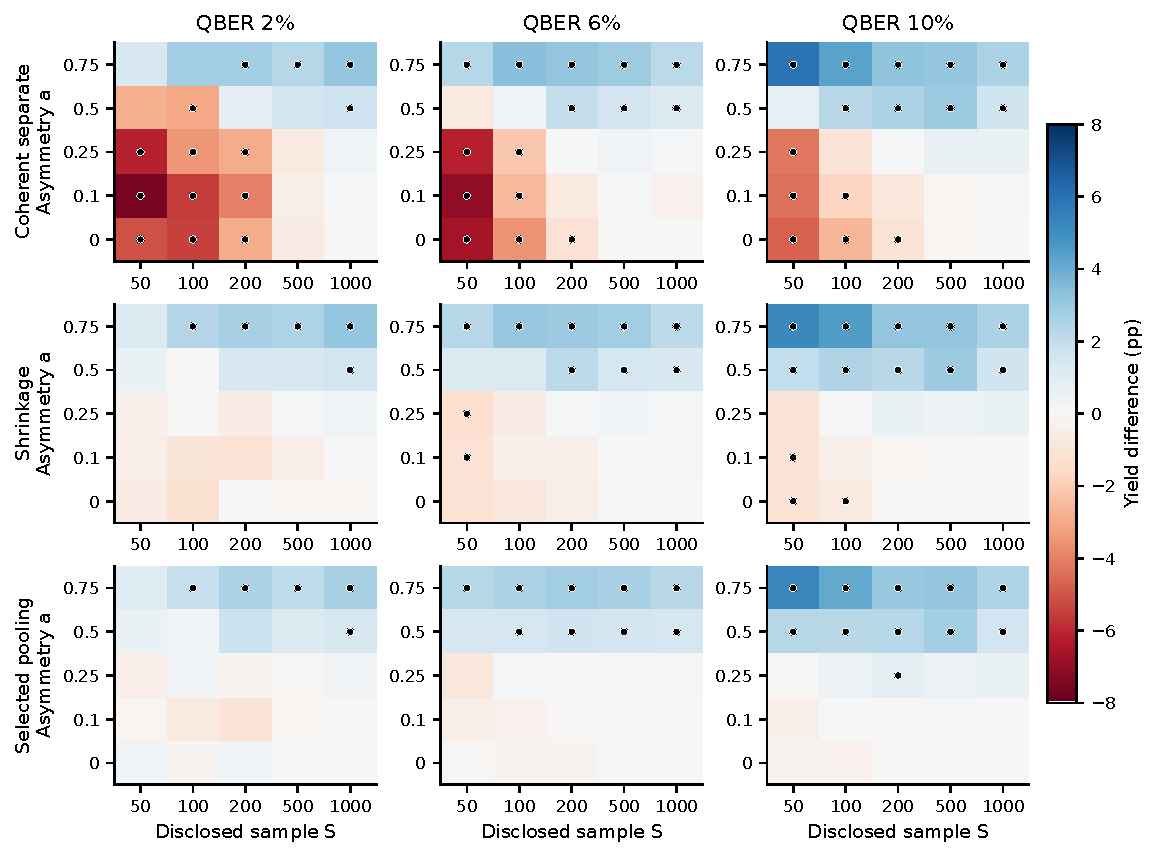
\includegraphics[width=0.98\linewidth]{images/asymmetry_map.pdf}
\caption{Confirmation yield changes relative to estimated pooling, in percentage points.
Rows compare coherent separate estimation, positive-part shrinkage, and the frozen
selected rule; columns give target QBER. Each panel includes all five asymmetries and
sample sizes, with 500 paired frames per cell. A dot marks a two-sided McNemar result
passing Holm correction over 75 cells for that comparator. Colour shows direction and
magnitude, not a confidence bound. Each QBER uses one fixed unseen matrix.}
\Description{Nine heatmaps show that separate estimates can harm weak-contrast cells,
while the selected pooling rule retains many gains and reduces these harms.}
\label{fig:asymmetry}
\end{figure}

Figure~\ref{fig:asymmetry} shows where the aggregate result comes from. Strong contrast
creates opportunities, but small samples make separate estimates costly. The selected
rule also reduces the average loss in equal-basis cells. Absence of a corrected significant harm is not
evidence of zero harm: at $Q=2\%,a=0.1,S=200$, the selected rule has nine harmed
and no rescued frames, a -1.029 pp difference, with Holm-adjusted $p=0.180$.
The rule improves the measured balance of benefits and costs on the confirmation
matrices; it does not dominate pooling frame by frame or condition by condition.

\FloatBarrier
\subsection{Transfer distinguishes fixed-code and policy outcomes}
\label{sec:transfer}
Figure~\ref{fig:transfer} reports every transfer condition. On a common code, three of
18 selected-prior matrix intervals lie above zero and two lie below zero. The losses
include the equal-basis Gallager condition at $n=4000,S=50$: -0.72 pp
(95\% interval [-1.03, -0.40]).
The confirmation result therefore does not establish harmless transfer to other codes.
At $n=16000$ with strong asymmetry, the fixed-code difference is 0.00 pp for Gallager
and +0.08 pp ([-0.15,+0.31]) for the irregular construction. A near-zero failure floor
can leave little room for a better prior to rescue frames at a fixed rate.

\begin{figure}[!htbp]
\centering
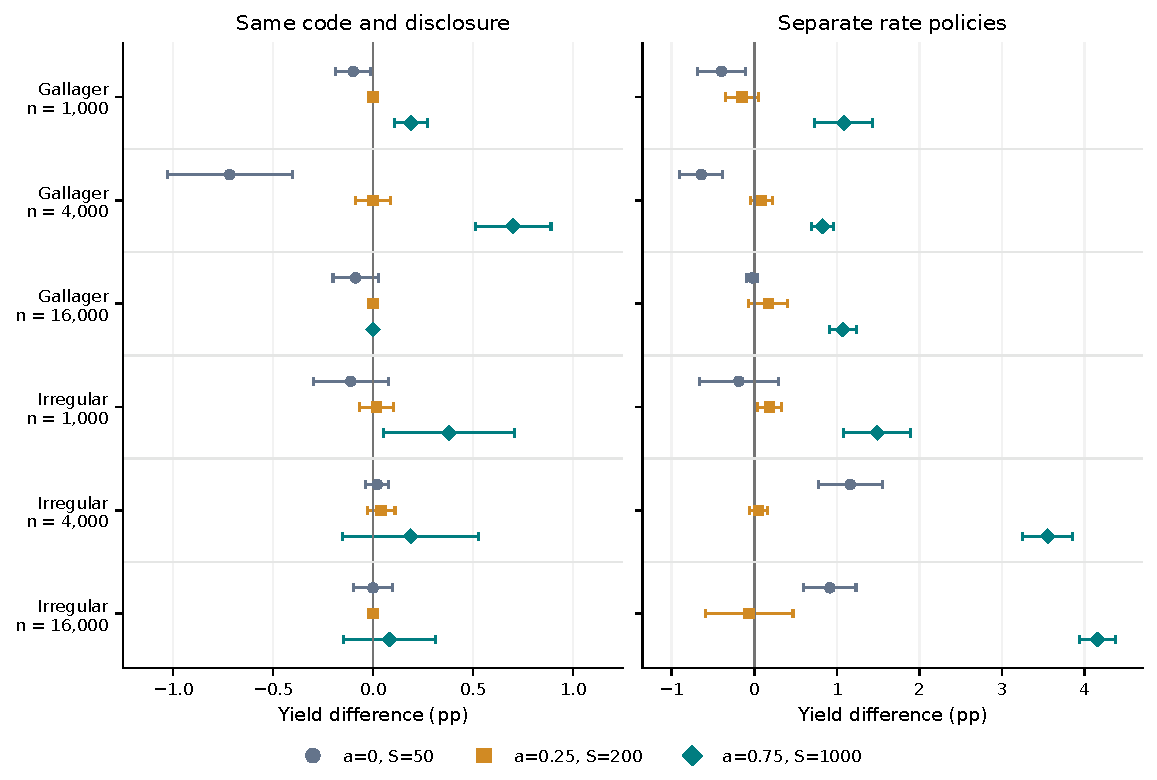
\includegraphics[width=0.97\linewidth]{images/transfer_comparison.pdf}
\caption{Transfer at 6\% QBER: fixed-code effects (left) and independently trained
rate-policy effects (right). Every family/length has three $(a,S)$ conditions.
Points are paired yield differences; bars are exploratory 95\% $t_4$ intervals across
five unseen matrix-library means, each based on 500 paired frames. The same input
frames are reused across code families. Intervals are not multiplicity-adjusted.}
\Description{Two forest plots distinguish small fixed-code gains and some losses from
larger but nonuniform rate-policy gains, across three block lengths and two code families.}
\label{fig:transfer}
\end{figure}
\FloatBarrier

Rate-policy gains are larger in several strong-asymmetry conditions, accompanied
by changes in syndrome length and recovery. The comparison measures both changes
together; it does not identify a causal effect of the prior on rate selection. At $n=16000,a=0.75,S=1000$, the
pipeline differences are +1.07 pp ([+0.91,+1.24]) for Gallager and +4.15 pp
([+3.94,+4.37]) for the irregular construction. These are effects of the prior together
with its independently learned rate policy, rather than isolated coding-efficiency
improvements at a fixed syndrome length.
The Gallager pipeline also loses 0.40 and 0.64 pp in its two shorter equal-basis
conditions. Conversely, the $n=16000$ irregular pipeline gains 0.92 pp with no
population basis contrast: its mean row fraction decreases from 0.45632 to 0.44004
while FER rises from 19.08\% to 19.40\%. This is direct evidence that policy
gains cannot be assigned to basis information alone. In the strong-asymmetry case,
the same family reduces its mean row fraction from 0.47106 to 0.42520 while FER
rises from 0.20\% to 0.48\%; Gallager instead improves FER from 0.60\% to zero.
Table~\ref{tab:absolutetransfer} reports absolute yields, efficiencies, and retained
batch timings; the supplement gives all transfer conditions. The two comparisons separate fixed-code effects from combined prior-and-selector
effects. A practical QKD rate selector also needs conservative margins for FER-model
uncertainty and drift, evaluated against frame-loss penalties; the fitted expected-yield
policy here does not certify such a margin.

The information benchmark puts these gains in context. At~\mbox{$Q=6\%,a=0.75$},
the pooled and basis-conditioned BSC entropies are 0.32744 and 0.29850 bits per
retained bit, so $G=0.02894$. Neither learned policy approaches those ideal floors:
the selected mean row fractions at $n=16000$ are 0.49330 for Gallager and 0.42520
for the irregular construction. A gain between two finite implementations is
therefore not a direct measure of the fraction of $G$ recovered.

To separate the recorded yield contributions, write $V_j=(n-m_j-64)/(n+S)$ and
$L_j=V_j(1-I_j)$ for each paired method $j\in\{\mathrm P,\mathrm S\}$. Then
\begin{equation}
 Y_{\mathrm S}-Y_{\mathrm P}
 =\underbrace{\frac{m_{\mathrm P}-m_{\mathrm S}}{n+S}}_{D}
 +\underbrace{L_{\mathrm P}-L_{\mathrm S}}_{R}.
 \label{eq:yielddecomposition}
\end{equation}
Here $D$ accounts for fewer syndrome rows and $R$ for the change in yield lost to
failed recovery. This is an exact accounting identity, not a causal attribution to
the prior: the fitted FER model, training variation, extrapolation, and tolerated
failure can all change the selected rows. The strong-asymmetry Gallager gain comprises +0.736 pp from
syndrome length and +0.337 pp from recovery; for the irregular construction these
terms are +4.316 and -0.163 pp (Appendix~\ref{app:rule},
Table~\ref{tab:yieldaccounting}). The latter disclosure gain exceeds the 2.724 pp
difference between ideal entropy-limited yields at this sample fraction because
the implementations have different excess disclosure above their respective floors.
It does not imply an information-theoretic gain larger than the channel provides.

\subsection{More estimation data can leave fewer recovered bits}
The fixed-total experiment asks whether a larger sample is worth sacrificing more of
the available block. With $n+S=2000$, both families attain their highest observed
selected-pipeline yield at $S=200$ among the five allocations. Increasing the sample
to $S=1000$ substantially reduces total yield even though the selected prior still
outperforms pooling at that allocation (Table~\ref{tab:sample}). Sample choice must therefore be assessed through
total yield, not probability-estimation accuracy alone. This finite grid does not
establish an optimal sample size beyond the evaluated policies and conditions.


\subsection{Physical noise determines which label is informative}
The information analysis in Section~\ref{sec:mechanism} predicts which conditioning
variables can help, but estimating them has a cost. In the matched-QBER controls,
gate-dependent and Pauli noise provide basis information; asymmetric readout instead
provides local-bit information despite $G=0$. Thermal relaxation provides both,
with the larger ideal increment coming from Bob's bit. These controls keep the
overall QBER at 6\%, so the distinction is not explained by an easier aggregate channel.

The transition-aware decoder estimates both directional error probabilities from
the disclosed sample and conditions on Bob's own retained bit. It never observes
Alice's undisclosed retained bit. This differs from the fully disclosed diagnostic
acquisition, where Alice's bit is an available stratum label. The same transition
law therefore supports different usable observations in the two tasks.

Readout controls illustrate the operational consequence: the transition-aware
prior improves yield by 0.29 pp for Gallager and 0.53 pp for the irregular family,
while the selected basis-only prior has no supported gain. Thermal controls also
favor transition-aware estimation. Under homogeneous noise, however, estimating
the unnecessary transition parameters harms recovery in both families.
Appendix~\ref{app:physical} gives the physical parameters, Bayes conversion to
decoder priors, and every matched-QBER outcome (Table~\ref{tab:physical}). The
physical model identifies which information could help; finite samples determine
whether it is worth estimating.

% Synthesize the decision implications without repeating each numerical result.
\section{Implications and Limits}
\label{sec:discussion}
The experiments connect three questions that aggregate QBER alone cannot answer:
what physical structure produces the errors, what the available observations
identify, and whether estimating that structure improves a finite-budget task.
These questions require different comparisons. Conditional entropy quantifies a
population opportunity; diagnostic MAE measures inference of a modeled residual;
reconciliation yield charges sampling, disclosure, and failed recovery. Keeping
those targets explicit allows the studies to support one argument without
implying a joint operational method.

\subsection{Preserving observations and acquiring new ones}
The cross-circuit study gives the central diagnostic result. PRIMARY provides a
direct residual path and benefits from retaining full transitions. Scheme A
remains identifiable from operating observations, and its precision ranking varies
with budget and interception: the scaling advantage at the anchor conditions
reverses in two weak-interception cells. B+ removes the operating contrast; a characterized scaling
intervention supplies identifying observations. Thus neither basis resolution nor noise
scaling is universally preferable. The useful decision is which observation
design identifies the target, under which assumptions, and at what precision
for the available signals.

The range comparison further shows why an acquisition must be specified by more
than its setting count. The two- and four-setting designs are much closer when
their ranges are matched; the widest tested range changes their ordering against
single-setting and calibrated estimators. These are finite candidate designs on
characterized depolarizing responses. The budget/interception grid broadens precision evidence within the model;
interior interpolation, one held-out scale, and three layouts do not establish
generality across devices. Hardware
use would require a characterized intervention, especially at large scale
factors, and sensitivity to loss, memory, preparation error, and correlated noise.

Profile likelihood adds a second distinction: uncertainty about the nuisance
devices and uncertainty about the residual need not be equally large. The
retained cohorts support useful residual precision despite broad device profiles,
but the empirical coverage remains conditional on the tested models and bounds.
Unknown unscaled readout changes what is identifiable, while drift can remove a
stationary target. Thermal and asymmetric-readout controls establish transition
structure for reconciliation; they do not validate the depolarizing diagnostic
response for those mechanisms.

\subsection{From conditional information to practical recovery}
The reconciliation study establishes a mechanism and its finite-sample boundaries.
It includes a nonzero-exposure circuit, a balanced control, a stronger decoder,
independent confirmation frames, and multiple transfer libraries. These checks
show why a conditional prior can help and why an estimated contrast can also harm.
At the longest blocks, fixed-code effects are negligible; larger gains come
through independently learned rate policies. The exact yield identity records
disclosure and failure contributions but cannot assign their causes to the prior.
The equal-basis pipeline gain makes that distinction observable.

The tested implementations do not establish a generally competitive coding
advance. Circuit-study $f_{\mathrm{EC}}$ values around 1.5--3.3 and substantial
excess disclosure at long blocks leave room for stronger constructions
\cite{elkouss2009,borisov2023}. One development realization leaves training
uncertainty unmeasured. The coupled transfer pairs at one QBER cannot separate
sample size from asymmetry. A competitive-code benchmark, repeated independent
development cohorts, and both priors evaluated across a common rate grid with
crossed selectors are the necessary tests of broader practical value. Five
evaluation libraries quantify matrix variation, not those missing sources of
uncertainty.

\subsection{Operational connection and security boundary}
The circuit classification illustrates how to assess further observation designs
before comparing their estimators. A joint estimator could retain bit-and-basis observations across scaling settings
and predict operating error probabilities for independent reconciliation frames.
Such a method would have to charge its acquisition cost, compare against full
single-setting observations, and test amortization under drift. A multi-parameter
noise model would also need enough independent observations or interventions to
identify its target. The present studies motivate these questions but establish
no joint diagnostic-and-decoding benefit. The zero-noise residual cannot replace
the operating error probabilities supplied to a decoder.

Bit-dependent errors also do not by themselves establish a new
privacy-amplification leakage term. Security requires the actual public transcript,
device assumptions, phase-error estimate, and Eve's side information to be treated
together~\cite{shor2000,tomamichel2012,rennerkoenig2005}. The conditional entropies
and yield here describe classical recovery; the residual describes a model-defined
disturbance. Neither substitutes for a finite-key security bound.

\section{Conclusion}
The implemented gate paths determine which BB84 observations identify a residual
disturbance. The proposition establishes operating-data identification in PRIMARY
and Scheme A, nonidentification in balanced B+, and four-setting sufficiency for
the latter's intercept. Unknown unscaled readout changes the identifiable target
to a combined residual, preventing an interception-only interpretation.

The precision study tests what identification alone cannot decide. Full operating
data favor PRIMARY across the tested grid, while Scheme A's scaling advantage
reverses in two weak-interception conditions. Explicit MAE-difference intervals,
matched acquisition ranges, and target profiles make the scope of those comparisons
visible. Their hardware use requires a characterized scaling law and accounting
for the cost and uncertainty of that characterization.

Reconciliation supplies supporting evidence for the cost of learning observable
structure. Pooling moderates finite-sample harms, but fixed-code benefits remain
conditional and the larger long-block gains include rate policies. Together, the
results classify residual identifiability for the specified BB84 implementations
and quantify the resulting acquisition--precision tradeoffs, supported by a
finite-sample recovery mechanism. They establish neither a general coding
improvement nor a secure-key result.

% Availability and declarations use the same scope as the reported experiments.
\section*{Data and Code Availability}
The computational supplement contains protocols, circuits, matrices, acquisition
and frame records, and analysis and verification scripts. It separates the circuit
study, pooling and transfer controls, matched-range diagnostics, full-observation
validation, and the budget/interception precision grid. Tables and figures are generated or checked against these records;
\texttt{absolute-transfer.csv} reports every absolute transfer outcome.
The accompanying archive, \texttt{bb84-reproducibility.zip}, contains
the complete source and five separately checksummed study components. From its
root, \texttt{python supplementary/reproduce\_final.py --mode build --compile}
regenerates the manuscript from retained records. The integrated \texttt{--mode analysis}
reruns the study analyses; each study's \texttt{--mode full} entry point regenerates
its simulations in a separate workspace. The archive's README gives these distinct workflows.

\section*{Conflicts of Interest}
The authors declare no conflicts of interest.

\FloatBarrier
\bibliographystyle{ACM-Reference-Format}
\bibliography{references}
\FloatBarrier
\clearpage
% Supplementary methods, complete operating points, and control comparisons.
% Generated table blocks are populated from the numerical results.
\appendix
\section{Experimental Inventory}
\label{app:inventory}
Table~\ref{tab:cohorts} separates independent inputs from their reuse across
estimators and decoders. Diagnostic blocks contain multiple strategies, each
charged its complete transmitted-signal budget. The precision grid uses fresh
acquisitions even at conditions shared with the cross-circuit study.

% BEGIN GENERATED COHORT_TABLE
\begin{table}[!htbp]
\centering
\small\setlength{\tabcolsep}{4pt}
\caption{Experimental map. Frame counts denote distinct inputs before reuse across priors, codes, or decoders. A diagnostic replicate block evaluates several fully budgeted acquisition strategies and produces no key. The 450 symmetric reference-calibration frames are additional. Detailed grids and reuse rules are given in the methods and supplement. Target profiles additionally reuse 2500 held-out-validation fitting records, without new acquisitions.}
\label{tab:cohorts}
\begin{tabular}{@{}lllr@{}}
\toprule
Cohort & Resource & Outcome & Inputs \\
\midrule
Circuit & $n=1000,S=200$ & FER and yield & 68,000 \\
Pooling/rate development & Varied $n,S$ & Frozen rules & 25,800 \\
Pooling confirmation & $n=1000$, varied $S$ & Fixed-code yield & 37,500 \\
Code transfer & $n=1000,4000,16000$ & Prior/policy yield & 22,500 \\
Sample allocation & $n+S=2000$ & Total yield & 12,500 \\
Physical controls & $n=1000,S=200$ & Conditional priors & 25,000 \\
Diagnostic reference/stress & Varied $T$ & Residual and coverage & 45,000 \\
Basis/range validation & Varied $T$; held-out setting & Residual and prediction & 31,000 \\
Full-data/circuit validation & $T=8000$ per strategy & Residual and coverage & 6,500 \\
Budget/interception validation & Varied $T,r$ & Precision contrasts & 40,500 \\
\bottomrule
\end{tabular}
\end{table}
% END GENERATED COHORT_TABLE
\FloatBarrier

\subsection{Uncertainty and computational checks}
Absolute FERs include failure counts and Wilson 95\% intervals~\cite{wilson1927}.
Exact two-sided McNemar tests use paired rescued/harmed frames. Holm correction covers
12 circuit cells separately for each decoder, and 75 confirmation cells separately for
each comparator. Paired bootstrap yield intervals (10,000 resamples) condition on each frozen matrix and
calibration choice; they do not include retraining uncertainty.

For transfer and physical/sample controls, the five matrix libraries are the units for
generalization. We report $t_4$ intervals on their paired mean yield differences, with
within-matrix frame uncertainty supplied separately. These exploratory intervals are
not adjusted across conditions. Zero observed discordance can collapse a bootstrap
interval at zero; it does not exclude rare harms. Grid means weight design cells equally
and are not population averages for a deployment.

Protocol-derived inventories count reused input frames only once. Independent
density-state calculations, decoder references, and retained-record checks verify
the implementation. Reproduction checks match all 1504 retained circuit-study arrays;
decoder audits cover every confirmation and transfer/control holdout and selected
development records. Diagnostic checks cover retained counts and budgets, density-state
responses, and independent reference fits. Fresh full runs match all 6670 retained range-validation arrays, all 1090
full-observation arrays, and all 3078 precision-grid arrays exactly. The full-observation study checks cross-circuit response
laws, analytic inverses, likelihood optima, and profile endpoints against
independent numerical references. The supplement specifies the
random-number generators, seeds, and exact verification scopes; cohort totals appear
in Appendix~\ref{app:rule}. Information benchmarks and yield decompositions are
descriptive calculations on the fixed evaluation records, not inputs used to tune
the selected rules. Entropies are checked both from joint probabilities and from
binary-transition formulas; the yield identity is checked for every paired frame.


\FloatBarrier
\section{Circuit Operating Points and Robustness}
\label{app:circuit}
\label{app:ablation}
The circuit study contains 6000 calibration frames, 24,000 main holdout frames,
6000 matrix-replication frames, 12,000 fixed-curve frames, and 20,000 channel
calibration/holdout frames. Reusing those frames across priors, decoders, and fixed-code
analyses does not create additional independent inputs. The matched comparison appears in Table~\ref{tab:matched};
Table~\ref{tab:operating} reports every calibrated operating point. The observed FER is below 1\% in all
12 main cells for both BP policies, although not every upper confidence bound is
below that threshold. The efficiencies describe this conservative finite-length
family and do not establish competitiveness with optimized QKD codes.

\subsection{Codes, calibration and circuit controls}
The circuit study uses a nested column-weight-three, progressive-edge-growth-style
family~\cite{hu2005}. Starting at 150 checks on 1000 variables, splitting a check into
two disjoint parts preserves nesting and gives $m=150,175,\ldots,900$. All 93 stored
matrices have full row rank. Layered sum-product belief propagation (BP) runs for at most 300 sweeps.
A stronger comparator adds full order-one ordered-statistics decoding (OSD)
\cite{fossorier1995} on nonconvergence or failed public verification, with the same search
budget for both priors. Simulator correctness never triggers the retry.

For each encoding and $Q\in\{0.02,0.06,0.10\}$, 500 calibration frames select the
smallest tested row count whose Wilson 95\% upper FER bound is at most 1\%, provided
all higher tested counts also pass. Pooled and shrinkage policies select separately.
Their choices are frozen before 2000 holdout frames per cell, giving 24,000 main
holdout frames. Fixed-code comparisons use the same shrinkage-selected matrix for
both priors; operating-policy comparisons allow their selected row counts to differ.
Two further matrix seeds, fixed-code curves, and link-noise controls complete the
68,000-frame circuit study.
A post hoc fixed-code sensitivity analysis replaces gate noise with isotropic link
noise at constant total QBER. It uses the gate-calibrated matrices to avoid the
near-zero failure floor of adaptive channel policies; channel outcomes do not
determine the selected matrices.


\begin{equation}
 f_{\mathrm{syn}}=\frac{m}{nh_2(Q)},\qquad
 f_{\mathrm{EC}}=\frac{m+64}{nh_2(Q)}.
 \label{eq:efficiency}
\end{equation}
Here $h_2(x)=-x\log_2x-(1-x)\log_2(1-x)$ is binary entropy, with $0\log_2 0=0$.
These disclosure efficiencies use the measured retained-block QBER in the
circuit study. Every transmitted syndrome row is charged, including dependent
rows. Authentication and privacy amplification are outside $Y$.
\subsection{Matched-code and operating comparisons}
\begin{table}[htbp]
\centering
\small\setlength{\tabcolsep}{3.2pt}
\caption{Matched-code comparisons at 10\% target QBER. Both priors use the shrinkage-selected matrix and the same 2000 frames. P/S denote pooled/shrinkage priors. Counts accompany absolute FER; R/H are rescued/harmed pairs. Ratios include paired bootstrap 95\% intervals when at least five pooled failures support estimation; a dash indicates an undefined or too-sparse ratio interval. Holm correction covers the 12 main cells separately for BP and BP+OSD.}
\label{tab:matched}
\begin{tabular}{@{}llcllccc@{}}
\toprule
Encoding & Decoder & $m$ & FER P (\%) & FER S (\%) & R/H & Ratio [95\% CI] & $p_{\rm Holm}$ \\
\midrule
Standard & BP & 625 & 112: 5.60 [4.67, 6.70] & 11: 0.55 [0.31, 0.98] & 102/1 & 0.098 [0.05, 0.16] & 2.5e-28 \\
Standard & BP+OSD & 625 & 88: 4.40 [3.59, 5.39] & 8: 0.40 [0.20, 0.79] & 81/1 & 0.091 [0.03, 0.16] & 4.1e-22 \\
A & BP & 650 & 33: 1.65 [1.18, 2.31] & 19: 0.95 [0.61, 1.48] & 16/2 & 0.576 [0.38, 0.78] & 0.014 \\
A & BP+OSD & 650 & 28: 1.40 [0.97, 2.02] & 13: 0.65 [0.38, 1.11] & 17/2 & 0.464 [0.26, 0.69] & 0.008 \\
B & BP & 675 & 3: 0.15 [0.05, 0.44] & 4: 0.20 [0.08, 0.51] & 0/1 & 1.333 [--] & 1 \\
B & BP+OSD & 675 & 1: 0.05 [0.01, 0.28] & 2: 0.10 [0.03, 0.36] & 0/1 & 2.000 [--] & 1 \\
B+ & BP & 700 & 0: 0.00 [0.00, 0.19] & 1: 0.05 [0.01, 0.28] & 0/1 & -- [--] & 1 \\
B+ & BP+OSD & 700 & 0: 0.00 [0.00, 0.19] & 1: 0.05 [0.01, 0.28] & 0/1 & -- [--] & 1 \\
\bottomrule
\end{tabular}
\end{table}
Operating-policy gains answer a different question because the selected syndrome lengths
can differ. In Scheme~A at 10\% QBER, pooled and shrinkage BP select 700 and 650
rows, respectively; their yield difference is +3.94 percentage points (pp), with paired
95\% interval [+3.83, +4.04]. The smaller syndrome comes with 19 failures versus
zero: shrinkage FER is 0.95\%, with Wilson interval [0.61\%,1.48\%]. Although
the point estimate is below 1\%, its upper bound exceeds the calibration criterion,
so the holdout does not establish the targeted reliability. The gain is largely a
disclosure effect conditional on that calibration. At 2\% QBER the same procedure loses 4.09 pp, and balanced B+ loses
2.00 pp at 10\%. Table~\ref{tab:operating} reports every operating cell, including
absolute FER and disclosure efficiency. These losses motivate a rule that can return
to pooling when the sample is uninformative.

\begin{table}[htbp]
\centering
\small\setlength{\tabcolsep}{3.2pt}
\caption{Main BP operating policies. Each cell has 2000 independent holdout frames. FER entries give failure counts, percentages, and Wilson 95\% intervals. P denotes pooled priors and S centred shrinkage. $m$ and $f_{\mathrm{EC}}$ are shown as P/S pairs. Yield differences and paired 95\% intervals are in percentage points. Target QBER labels denote generator expectations.}
\label{tab:operating}
\begin{tabular}{@{}lcccllc@{}}
\toprule
Encoding & $Q$ (\%) & $m$ P/S & $f_{\mathrm{EC}}$ P/S & FER P (\%) & FER S (\%) & $\Delta Y$ (pp) \\
\midrule
Standard & 2 & 400/400 & 3.29/3.29 & 0: 0.00 [0.00, 0.19] & 0: 0.00 [0.00, 0.19] & +0.00 [+0.00, +0.00] \\
Standard & 6 & 550/525 & 1.88/1.80 & 0: 0.00 [0.00, 0.19] & 1: 0.05 [0.01, 0.28] & +2.07 [+2.03, +2.08] \\
Standard & 10 & 700/625 & 1.63/1.47 & 1: 0.05 [0.01, 0.28] & 11: 0.55 [0.31, 0.98] & +6.12 [+6.03, +6.19] \\
A & 2 & 300/350 & 2.57/2.92 & 4: 0.20 [0.08, 0.51] & 1: 0.05 [0.01, 0.28] & -4.09 [-4.16, -3.98] \\
A & 6 & 550/525 & 1.87/1.80 & 3: 0.15 [0.05, 0.44] & 5: 0.25 [0.11, 0.58] & +2.05 [+1.96, +2.13] \\
A & 10 & 700/650 & 1.63/1.52 & 0: 0.00 [0.00, 0.19] & 19: 0.95 [0.61, 1.48] & +3.94 [+3.83, +4.04] \\
B & 2 & 300/300 & 2.56/2.56 & 9: 0.45 [0.24, 0.85] & 7: 0.35 [0.17, 0.72] & +0.05 [-0.05, +0.16] \\
B & 6 & 525/525 & 1.80/1.80 & 8: 0.40 [0.20, 0.79] & 9: 0.45 [0.24, 0.85] & -0.02 [-0.05, +0.00] \\
B & 10 & 675/675 & 1.58/1.58 & 3: 0.15 [0.05, 0.44] & 4: 0.20 [0.08, 0.51] & -0.01 [-0.03, +0.00] \\
B+ & 2 & 375/375 & 3.12/3.12 & 0: 0.00 [0.00, 0.19] & 0: 0.00 [0.00, 0.19] & +0.00 [+0.00, +0.00] \\
B+ & 6 & 525/525 & 1.81/1.81 & 7: 0.35 [0.17, 0.72] & 7: 0.35 [0.17, 0.72] & +0.00 [+0.00, +0.00] \\
B+ & 10 & 675/700 & 1.58/1.63 & 9: 0.45 [0.24, 0.85] & 1: 0.05 [0.01, 0.28] & -2.00 [-2.06, -1.92] \\
\bottomrule
\end{tabular}
\end{table}


Figure~\ref{fig:exposure} compares path-model predictions with measured basis probabilities.
Figure~\ref{fig:curves} evaluates fixed codes across QBER, avoiding changes in code profile
within a curve. Their purpose is to expose the mechanism and operating regime rather than
maximize a single failure ratio.

\begin{figure}[htbp]
\centering
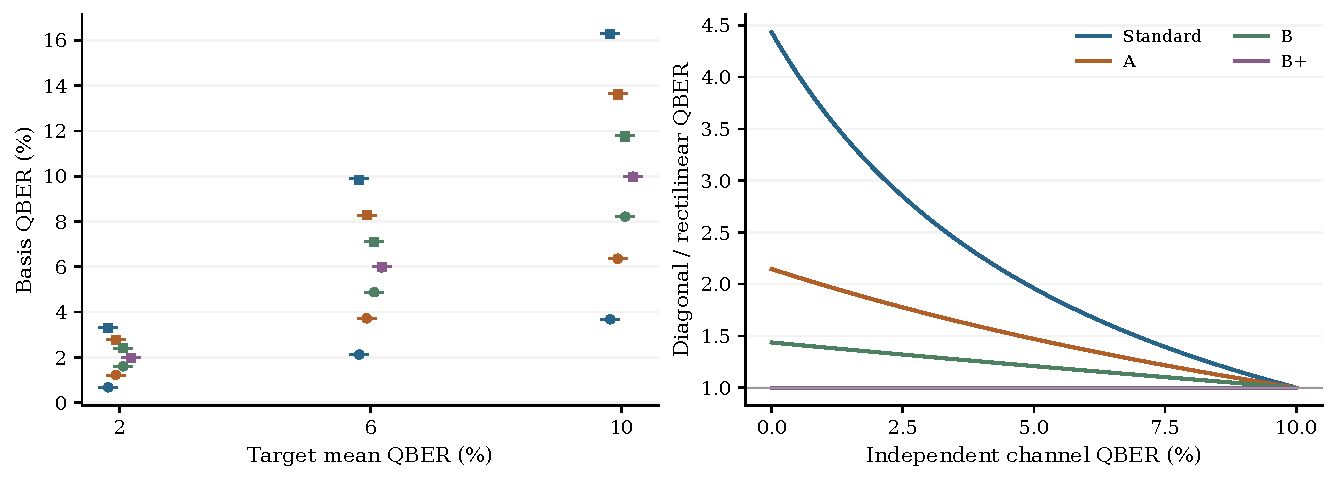
\includegraphics[width=0.94\linewidth]{images/gate_exposure.pdf}
\caption{Left: measured basis QBERs across the main holdout frames; circles indicate rectilinear and squares diagonal. Colors follow Standard, A, B, and B+ as in the legend at right. Short horizontal marks give exact gate-model predictions. Wilson 95\% error bars are smaller than most markers because each point pools approximately 1.2 million bits. Right: predicted attenuation of the basis ratio when channel noise replaces gate noise at fixed 10\% total QBER.}
\Description{Basis error probabilities agree with gate-count predictions; independent channel noise drives each diagonal-to-rectilinear ratio to one.}
\label{fig:exposure}
\end{figure}

\begin{figure}[htbp]
\centering
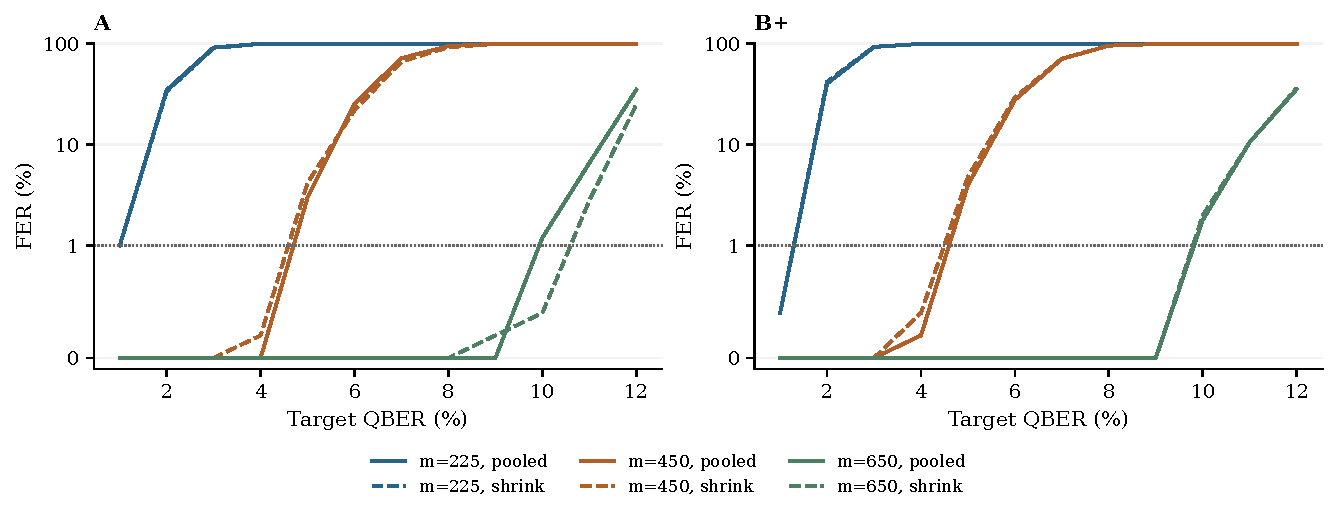
\includegraphics[width=0.94\linewidth]{images/fixed_code_curves.pdf}
\caption{Fixed-code BP curves, with 500 independent frames at each QBER. Solid lines use pooled priors and dashed lines use centred shrinkage. Each color is one matrix, reused across QBER. The dotted line marks 1\% FER; the vertical axis is linear below 1\% and logarithmic above it. Zero observed failures have Wilson 95\% upper bound 0.76\%. Full counts accompany the curves.}
\Description{FER-versus-QBER transitions for three fixed matrices in Scheme A and balanced control B+.}
\label{fig:curves}
\end{figure}

Table~\ref{tab:ablation} compares all four estimators at the same shrinkage-selected
matrix in the 10\% cells. Table~\ref{tab:replication} transfers the frozen row counts to
two fresh matrices and independent frames. Each comparison therefore isolates estimator
or matrix variation without using the evaluation frame to retune the rate.
\begin{table}[htbp]
\centering
\small\setlength{\tabcolsep}{3.2pt}
\caption{Prior-estimation ablation at 10\% QBER. Entries are exact failures out of 2000 paired frames on one common matrix in each cell. P is pooled Jeffreys; J is separate Jeffreys; C is coherent unshrunk; S is centred shrinkage. Complete counts at 2\% and 6\% accompany the same analysis.}
\label{tab:ablation}
\begin{tabular}{@{}llccccc@{}}
\toprule
Encoding & Decoder & $m$ & P & J & C & S \\
\midrule
Standard & BP & 625 & 112 & 10 & 10 & 11 \\
Standard & BP+OSD & 625 & 88 & 6 & 8 & 8 \\
A & BP & 650 & 33 & 13 & 12 & 19 \\
A & BP+OSD & 650 & 28 & 13 & 10 & 13 \\
B & BP & 675 & 3 & 5 & 6 & 4 \\
B & BP+OSD & 675 & 1 & 4 & 5 & 2 \\
B+ & BP & 700 & 0 & 2 & 2 & 1 \\
B+ & BP+OSD & 700 & 0 & 2 & 2 & 1 \\
\bottomrule
\end{tabular}
\end{table}

\begin{table}[htbp]
\centering
\small\setlength{\tabcolsep}{3.2pt}
\caption{Additional matrix seeds at 10\% target QBER. Each seed/encoding uses 1000 fresh frames. Both priors use the shrinkage row count from independent seed-11 calibration. Entries show failure counts, FER percentages, and Wilson 95\% intervals. OSD denotes BP+OSD.}
\label{tab:replication}
\begin{tabular}{@{}clcllll@{}}
\toprule
Seed & Encoding & $m$ & BP P (\%) & BP S (\%) & OSD P (\%) & OSD S (\%) \\
\midrule
29 & Standard & 625 & 62: 6.20 [4.87, 7.87] & 5: 0.50 [0.21, 1.17] & 57: 5.70 [4.43, 7.31] & 4: 0.40 [0.16, 1.02] \\
29 & A & 650 & 17: 1.70 [1.06, 2.71] & 13: 1.30 [0.76, 2.21] & 13: 1.30 [0.76, 2.21] & 11: 1.10 [0.62, 1.96] \\
29 & B+ & 700 & 0: 0.00 [0.00, 0.38] & 1: 0.10 [0.02, 0.56] & 0: 0.00 [0.00, 0.38] & 1: 0.10 [0.02, 0.56] \\
47 & Standard & 625 & 43: 4.30 [3.21, 5.74] & 7: 0.70 [0.34, 1.44] & 36: 3.60 [2.61, 4.94] & 7: 0.70 [0.34, 1.44] \\
47 & A & 650 & 19: 1.90 [1.22, 2.95] & 8: 0.80 [0.41, 1.57] & 12: 1.20 [0.69, 2.09] & 7: 0.70 [0.34, 1.44] \\
47 & B+ & 700 & 0: 0.00 [0.00, 0.38] & 1: 0.10 [0.02, 0.56] & 0: 0.00 [0.00, 0.38] & 1: 0.10 [0.02, 0.56] \\
\bottomrule
\end{tabular}
\end{table}



\FloatBarrier
Table~\ref{tab:channel} retains the same gate-only calibrated matrices while an independent
isotropic channel replaces gate noise at fixed total QBER. The zero-channel row reuses
main holdout frames. The adaptive channel-policy analysis and paired uncertainty are
provided in the computational supplement.

\subsection{A basis-independent channel attenuates the signal}
We insert an independent depolarizing link between preparation and reception, with bit-error
probability $c$ in either basis. Isotropy allows this channel to be commuted to the end of
the path for calculation. The resulting basis probabilities are
\begin{equation}
 p_z^{\mathrm{tot}}=c+(1-2c)p_z^{\mathrm{gate}},\qquad z\in\{r,d\}.
 \label{eq:channel}
\end{equation}
At fixed total QBER $Q$, the average gate contribution is $(Q-c)/(1-2c)$. Increasing $c$
therefore reduces the basis contrast, reaching zero at $c=Q$. This control isolates noise
composition from an increase in overall decoding difficulty.

The link-noise control also narrows the mechanism. At fixed 10\% total QBER and
fixed disclosure, replacing gate noise with isotropic channel noise removes the basis
contrast. At the pure-channel endpoint, the shrinkage and pooled decoders fail on 110 and 98 frames, respectively,
in Standard, and on 33 and 27 in A (Table~\ref{tab:channel}). This fixed-code sensitivity analysis demonstrates
why an estimate of basis contrast can become a liability when that contrast disappears.

\begin{table}[!htbp]
\centering
\small\setlength{\tabcolsep}{3.2pt}
\caption{Fixed-code channel-composition BP controls at 10\% total target QBER. Each cell has 2000 independent holdout frames. The zero-channel points reuse the main cohort. FER entries show counts, percentages, and Wilson 95\% intervals.}
\label{tab:channel}
\begin{tabular}{@{}lcc ll@{}}
\toprule
Encoding & $c$ (\%) & $m$ & FER P (\%) & FER S (\%) \\
\midrule
Standard & 0.0 & 625 & 112: 5.60 [4.67, 6.70] & 11: 0.55 [0.31, 0.98] \\
Standard & 2.5 & 625 & 98: 4.90 [4.04, 5.94] & 31: 1.55 [1.09, 2.19] \\
Standard & 5.0 & 625 & 105: 5.25 [4.36, 6.32] & 86: 4.30 [3.50, 5.28] \\
Standard & 7.5 & 625 & 94: 4.70 [3.86, 5.72] & 93: 4.65 [3.81, 5.66] \\
Standard & 10.0 & 625 & 98: 4.90 [4.04, 5.94] & 110: 5.50 [4.58, 6.59] \\
A & 0.0 & 650 & 33: 1.65 [1.18, 2.31] & 19: 0.95 [0.61, 1.48] \\
A & 2.5 & 650 & 26: 1.30 [0.89, 1.90] & 24: 1.20 [0.81, 1.78] \\
A & 5.0 & 650 & 23: 1.15 [0.77, 1.72] & 24: 1.20 [0.81, 1.78] \\
A & 7.5 & 650 & 25: 1.25 [0.85, 1.84] & 27: 1.35 [0.93, 1.96] \\
A & 10.0 & 650 & 27: 1.35 [0.93, 1.96] & 33: 1.65 [1.18, 2.31] \\
\bottomrule
\end{tabular}
\end{table}
% The lookup rule and rate policies are fixed before evaluation.
\section{Conditional Information, Pooling and Transfer}
\label{app:rule}
\subsection{Information benchmarks}\label{app:information}
For asymptotically reliable one-way reconciliation with known channel probabilities,
conditional entropy supplies the classical benchmark~\cite{slepian1973,elkouss2011}.
The information made available by retaining the basis is
\begin{equation}
 G=H(A\mid B)-H(A\mid B,Z)=I(A;Z\mid B)\geq0.
 \label{eq:information}
\end{equation}
For basis-conditioned binary symmetric channels (BSCs),
\begin{equation}
 H(A\mid B,Z)=\sum_z P(Z=z)h_2(p_z),\qquad
 G=h_2(Q)-\sum_z P(Z=z)h_2(p_z).
 \label{eq:mixtureentropy}
\end{equation}
These are established information identities, not predictions of finite-length BP
performance. The BSC reduction is inappropriate when error probabilities depend
on Alice's bit; then we compute both entropies from the full transition law.

There is also a distinction between knowing the basis and using the full channel.
For error bit $U=A\oplus B$, a basis-only Bernoulli prior has ideal expected
log loss $H(U\mid Z)$, whereas a transition-aware prior can attain
$H(U\mid B,Z)=H(A\mid B,Z)$. Their difference
$D_B=I(U;B\mid Z)$ measures the additional information in Bob's local bit after
conditioning on basis. It is distinct from $G$, whose comparator already uses $B$.
In an asymmetric channel, observing $B=0$ or $B=1$ can change the probability
that a position is erroneous even at fixed $Z$. Thus asymmetric readout can
have $D_B>0$ while $G=0$; thermal relaxation can provide both kinds of information.
These are population log-loss opportunities, not guaranteed finite-sample yield gains.
Neither quantity establishes what an eavesdropper learns.

% BEGIN GENERATED INFORMATION_TABLE
\begin{table}[!htbp]
\centering
\small\setlength{\tabcolsep}{4pt}
\caption{Channel information for the five B+ controls matched to $Q=6\%$. Values are bits per retained bit, computed from the stored transition probabilities with uniform input bits and bases. $G=I(A;Z\mid B)$ is the basis benefit relative to a decoder already using $B$; $D_B=I(U;B\mid Z)$ is the extra ideal error-prior log-loss reduction from Bob\textquotesingle s bit after conditioning on basis. These are distinct quantities and are not added together.}
\label{tab:information}
\begin{tabular}{@{}lrrrr@{}}
\toprule
Mechanism & $H(A\mid B)$ & $H(A\mid B,Z)$ & $G$ & $D_B$ \\
\midrule
Homogeneous & 0.32744 & 0.32744 & 0.00000 & 0.00000 \\
Gate-dependent & 0.32705 & 0.30538 & 0.02166 & 0.00088 \\
Pauli link & 0.32744 & 0.30977 & 0.01768 & 0.00000 \\
Thermal & 0.29886 & 0.29257 & 0.00629 & 0.03274 \\
Readout & 0.29758 & 0.29758 & 0.00000 & 0.02986 \\
\bottomrule
\end{tabular}
\end{table}
% END GENERATED INFORMATION_TABLE


The matched physical controls distinguish basis information from local-bit
information at fixed QBER. Gate-dependent and Pauli noise provide a basis
benefit; readout supplies local-bit information even when the basis benefit
vanishes. Thermal relaxation supplies both. The transition-aware priors in
Appendix~\ref{app:physical} test these differences using finite disclosed samples.

\subsection{Prior estimation and a sample-only pooling rule}
\label{app:reconmethods}
\label{sec:methods}
Let $E_z$ errors be observed among $S_z$ disclosed bits in basis $z$, with
$E=E_r+E_d$ and $S=S_r+S_d$. Define
\begin{equation}
 \widehat p=\frac{E+1/2}{S+1},\qquad
 \widetilde p=\frac ES,\qquad
 \widetilde p_z=\frac{E_z}{S_z}.
 \label{eq:pool}
\end{equation}
Separate Jeffreys estimates introduce a total of one pseudo-error across two classes,
whereas the pooled estimate introduces one half. To avoid crediting extra smoothing to
basis information, our main family retains one common centre:
\begin{equation}
 \widehat p_z(\lambda)=\widehat p+\lambda(\widetilde p_z-\widetilde p),
 \qquad 0\leq\lambda\leq1.
 \label{eq:shrink}
\end{equation}
Its sample-weighted mean is $\widehat p$ before clipping. We call $\lambda=0$ pooled
and $\lambda=1$ coherent separate estimation. An absent class takes the pooled raw
proportion. The positive-part shrinkage comparator uses
\begin{equation}
 d=\widetilde p_d-\widetilde p_r,\quad
 v=\widehat p(1-\widehat p)(S_r^{-1}+S_d^{-1}),\quad
 \lambda_{\mathrm{sh}}=\max\{0,1-v/d^2\},
 \label{eq:weight}
\end{equation}
with weight zero when $d=0$ or a class is absent. This is a plug-in heuristic, not a
dominance guarantee. Separate-Jeffreys and coherent-separate ablations in the circuit
study distinguish centring from shrinkage.

The distinct \emph{selected pooling rule} learns a 24-entry lookup table
from development frames. It chooses $\lambda\in\{0,0.25,0.5,0.75,1\}$ from
sample-only features $S,\widehat p,d^2/v$, maximizing a conservative paired-yield
score. The rule is frozen before confirmation. The rule specification below gives
the bins, score, tie handling, and every selected weight. This is a training
heuristic, not a post-selection confidence guarantee.

Bob's error-vector prior is $L_i=\log[(1-\widehat p_{z_i})/\widehat p_{z_i}]$.
The decoder clips probabilities to $[10^{-6},0.499]$. The lower limit avoids infinite
log odds; the upper limit additionally assumes that a bit is more likely correct
than flipped. This is a model restriction, not a numerical necessity. A retained-record
check finds that neither limit is active for any of the 37,500 confirmation frames
or 25,000 distinct physical-control frames, including transition-aware estimates
whose largest raw probability is 0.2572. These results therefore do not test channels
that require negative error-prior log odds. Each frame's sample is disjoint from its decoded bits. Population asymmetry and true error
probabilities are forbidden inputs to the deployed rule. Oracle pooled and oracle
basis priors are reported only as benchmarks for the cost of learning probabilities.

\subsection{Confirmation design}
To vary sample size independently of a circuit-specific contrast, the confirmation study uses
basis-conditioned BSCs with $p_r=Q(1-a)$ and $p_d=Q(1+a)$. Its 75 cells cross
$Q\in\{0.02,0.06,0.10\}$, $a\in\{0,0.1,0.25,0.5,0.75\}$, and
$S\in\{50,100,200,500,1000\}$ at $n=1000$. Independent symmetric reference
calibration uses 450 frames to select $m=250,475,600$ at the three QBERs, respectively,
near a 10\% FER transition. A 15,000-frame pilot learns the pooling table on matrix
seed 11. Confirmation uses 37,500 new frames and unseen matrix seed 29, with 500
frames per cell, but retains the pilot's entire $(Q,a,S)$ grid and the same $m$
values. It therefore tests replication within the development design, not generalization
to new conditions or code families. The transfer experiment in
Section~\ref{sec:transfer} supplies that distinct test. These sensitivity conditions
also differ from the circuit study's low-FER operating points.

\subsection{Unseen codes, longer blocks, and fixed resources}
Transfer uses a three-partition Gallager construction and an irregular construction with
the variable-degree fractions of Elkouss et al.~\cite{elkouss2009}, converted from edge
to node fractions. A bounded local-cycle search and degree-balanced checks realize the
latter. Its check distribution differs from the published ensemble, and row fractions
above 0.50 reuse the 0.50 variable-degree profile. No published asymptotic threshold or
state-of-the-art efficiency is attributed to these realizations.

Development libraries use seeds 101 and 103 at $n=1000,4000,16000$; five unseen
libraries use seeds 211, 223, 227, 229, and 233. All confirmation and transfer/control
decoders use layered sum-product BP with 100 sweeps and the same verification rule.
OSD is evaluated only in the circuit study. The selected prior and the transfer policies
are not claimed to retain their effects under an OSD retry.

Two complementary comparisons are retained. A fixed-code comparison uses one common
matrix and disclosure, chosen to maximize pooled-decoder yield on independent 6\%-QBER
development data spanning $a=0,0.5$ and $S=50,200,1000$. A pipeline comparison lets
each method choose its syndrome length from the same row-fraction pool, 0.15 to 0.80
in steps of 0.05. Both use the same sample features, ridge-logistic training procedure,
and development budget to predict FER and maximize expected $Y$ before decoding.
Development evaluates entropy-margin subsets of this pool; predictions for some
feature/rate combinations therefore extrapolate beyond training support. The policies
are comparable learned selectors, not globally optimal rate adaptation.

At $Q=0.06$, transfer crosses the three block lengths with
$(a,S)=(0,50),(0.25,200),(0.75,1000)$. Asymmetry and sample size vary together,
so this transfer design does not estimate their separate effects or test unseen QBERs. A pilot-based precision calculation selects
500 paired frames per matrix and condition. A separate fixed-total experiment keeps
$n+S=2000$, $Q=0.06$, and $a=0.5$, transfers the policies without retuning, and
constructs matrices at the exact retained length $n=2000-S$. No padded bits are
counted as data. Physical controls use B+ at $n=1000,S=200$ with five noise
mechanisms, both at fixed parameters and after matching the overall QBER to 6\%.
Their transition laws and the Bob-bit-conditioned prior are specified in
Appendix~\ref{app:physical}.

\subsection{Frozen pooling rule}

Table~\ref{tab:rule} gives every weight in the frozen lookup rule. The lower sample bin
includes $S=100$; a QBER or squared-contrast value exactly at a cut point enters the
upper bin. All bin inputs come from the current frame's disclosed sample. Weights were
selected on 15,000 pilot frames and were not retuned on the 37,500 confirmation frames
or any transfer/control outcomes. The pilot score selects among five weights within
each bin. For the $N_b$ pilot frames assigned to bin $b$, let
$\Delta_i(\lambda)=Y_i(\lambda)-Y_i(0)$ be the paired yield difference, using
the same frame and code for both weights and the yield in Eq.~\eqref{eq:yield}.
For $N_b>1$, the selection score is
\begin{equation}
 L_b(\lambda)=\overline\Delta_b(\lambda)
 -1.96\sqrt{\frac{\sum_{i\in b}[\Delta_i(\lambda)-\overline\Delta_b(\lambda)]^2}
 {N_b(N_b-1)}}.
 \label{eq:poolingscore}
\end{equation}
This uses the sample standard deviation of paired differences divided by
$\sqrt{N_b}$. The chosen weight maximizes $L_b$ over the ascending grid
$(0,0.25,0.5,0.75,1)$; exact ties choose the smallest weight. For $N_b\leq1$
all scores are set to zero, selecting pooling. The 1.96 penalty is a development
heuristic, not a simultaneous or post-selection confidence guarantee.
The implementation is \texttt{extensions/pilot.py}, function \texttt{train},
under \texttt{supplementary/}; the stored rule retains every bin count and score.

% BEGIN GENERATED RULE_TABLE
\begin{table}[!htbp]
\centering
\small\setlength{\tabcolsep}{4pt}
\caption{Frozen partial-pooling weights $\lambda$ selected using pilot data only. Columns give the squared sample contrast $d^2/v$.}
\label{tab:rule}
\begin{tabular}{@{}llrrrr@{}}
\toprule
Sample & Pooled estimate & $<1$ & $[1,4)$ & $[4,9)$ & $\geq9$ \\
\midrule
$S\leq100$ & $\widehat p<0.04$ & 0.25 & 0.25 & 0 & 0 \\
$S\leq100$ & $0.04\leq\widehat p<0.08$ & 0 & 0.25 & 0.25 & 0 \\
$S\leq100$ & $\widehat p\geq0.08$ & 0 & 0.5 & 0.5 & 0.5 \\
$S>100$ & $\widehat p<0.04$ & 0 & 0.5 & 0.5 & 1 \\
$S>100$ & $0.04\leq\widehat p<0.08$ & 0 & 0 & 0.75 & 0.75 \\
$S>100$ & $\widehat p\geq0.08$ & 0 & 0.5 & 0.5 & 0.75 \\
\bottomrule
\end{tabular}
\end{table}
% END GENERATED RULE_TABLE

The transfer policies use nine standardized features: pooled entropy, pooled QBER,
$\log(1+\min\{100,d^2/v\})$, $S^{-1/2}$, $\log(n/1000)$, row fraction
$\beta=m/n$, $\beta-h_2(\widehat p)$, its square, and pooled entropy times the
log-contrast feature. Each family/prior has a logistic FER model with an unpenalized
intercept and ridge coefficient one for every other standardized coefficient.
Development crosses three QBERs, two asymmetries, three sample sizes, three lengths,
and two library seeds, with 100 input frames per condition. Candidate row fractions
are the shared-pool values nearest $\alpha h_2(Q)$ for
$\alpha\in\{1.1,1.35,1.6,1.9\}$. Generator $Q$ defines this development design;
the deployed features use sampled $\widehat p$. The model then predicts every
candidate in the full row-fraction pool before choosing a test-frame code.

This development design produces 10,800 independent input frames. The other cohorts
comprise 15,000 pilot, 37,500 confirmation, 22,500 transfer,
12,500 fixed-total, and 25,000 physical-control frames, for 123,300 in total.
Matching inputs across families, methods, or candidate rates are counted once.
The 450 reference-calibration frames are additional. Reusing the input frames across
decoders and policies produces 1,163,400 outputs; the diagnostic reference-and-stress cohort
contains 45,000 acquisition replicate blocks. Basis/range and held-out validation
add 31,000 blocks. Full-observation validation adds 6500 blocks; its target-profile
analysis reuses 2500 fitting records from held-out validation. Acquisition counts
and reuse rules are specified in Appendix~\ref{app:diagnostic}.

\subsection{Complete confirmation results}
\label{app:confirmation}
The table and heatmap retain all 75 confirmation conditions and every comparator.
The selected rule's worst cell, at $Q=2\%,a=0.1,S=200$, has nine harmed
and no rescued frames: a -1.029 pp yield difference with Holm-adjusted
$p=0.180$. Its equal-cell mean gain is 0.813 pp, compared with 1.804 pp
for the oracle basis prior. Both quantities condition on the repeated
development grid and the unseen confirmation matrix.
% BEGIN GENERATED ASYMMETRY_TABLE
\begin{table}[!htbp]
\centering
\small\setlength{\tabcolsep}{4pt}
\caption{Confirmation against estimated pooling. Supported gains and harms pass a two-sided exact McNemar test with Holm correction across 75 cells separately for each method. All cells have 500 paired frames. Means weight cells equally; the equal-basis column uses the 15 cells with $a=0$. Yield differences are in percentage points.}
\label{tab:asymmetry}
\begin{tabular}{@{}lrrrr@{}}
\toprule
Prior & Gains /75 & Harms /75 & Mean $\Delta Y$ & $a=0$ mean \\
\midrule
Coherent separate & 21 & 23 & -0.509 & -2.297 \\
Positive-part shrinkage & 23 & 5 & +0.669 & -0.444 \\
Selected pooling & 25 & 0 & +0.813 & -0.056 \\
Oracle pooled & 6 & 0 & +0.413 & +0.376 \\
Oracle basis & 41 & 0 & +1.804 & +0.376 \\
\bottomrule
\end{tabular}
\end{table}
% END GENERATED ASYMMETRY_TABLE
\begin{figure}[!htbp]
\centering
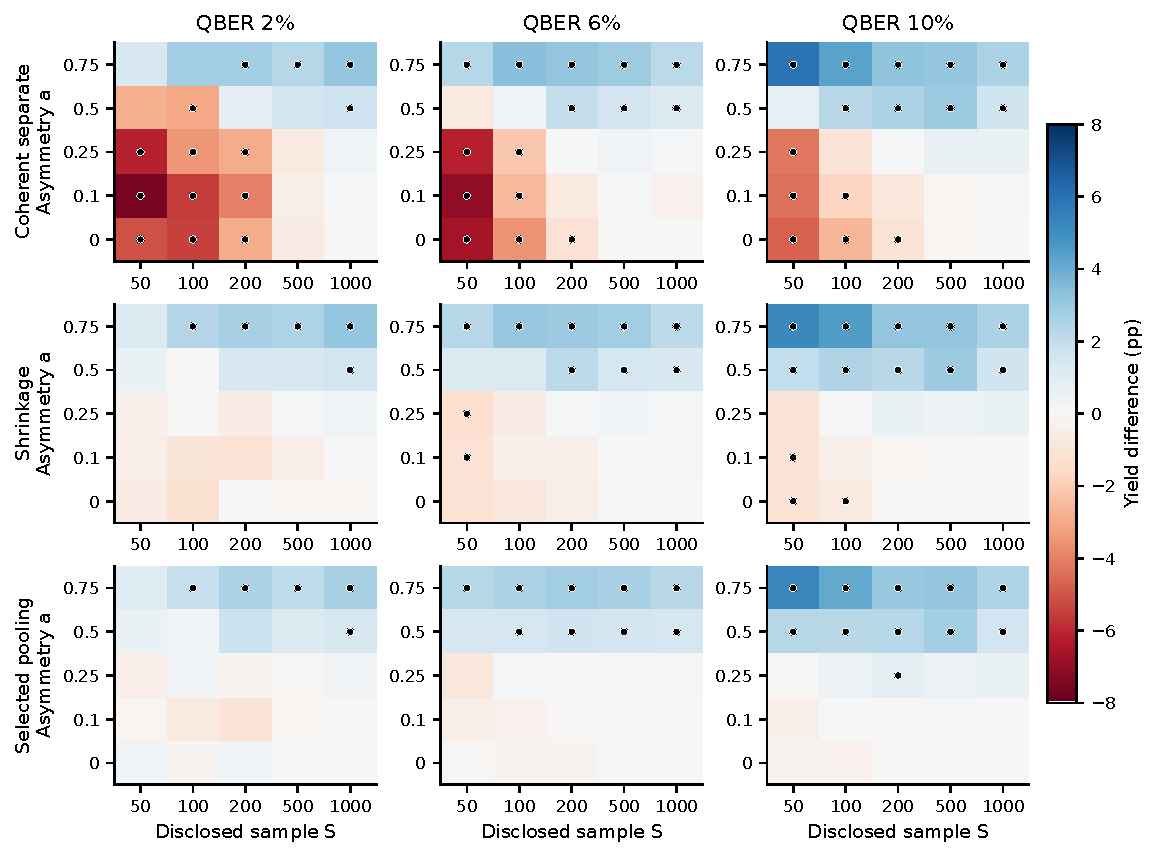
\includegraphics[width=0.98\linewidth]{images/asymmetry_map.pdf}
\caption{Confirmation yield changes relative to estimated pooling, in percentage points.
Rows compare coherent separate estimation, positive-part shrinkage, and the frozen
selected rule; columns give target QBER. Each panel includes all five asymmetries and
sample sizes, with 500 paired frames per cell. A dot marks a two-sided McNemar result
passing Holm correction over 75 cells for that comparator. Colour shows direction and
magnitude, not a confidence bound. Each QBER uses one fixed unseen matrix.}
\Description{Nine heatmaps show that separate estimates can harm weak-contrast cells,
while the selected pooling rule retains many gains and reduces these harms.}
\label{fig:asymmetry}
\end{figure}
\subsection{Transfer accounting and absolute outcomes}
The information benchmark puts these gains in context. At~\mbox{$Q=6\%,a=0.75$},
the pooled and basis-conditioned BSC entropies are 0.32744 and 0.29850 bits per
retained bit, so $G=0.02894$. Neither learned policy approaches those ideal floors:
the selected mean row fractions at $n=16000$ are 0.49330 for Gallager and 0.42520
for the irregular construction. A gain between two finite implementations is
therefore not a direct measure of the fraction of $G$ recovered.

To separate the recorded yield contributions, write $V_j=(n-m_j-64)/(n+S)$ and
$L_j=V_j(1-I_j)$ for each paired method $j\in\{\mathrm P,\mathrm S\}$. Then
\begin{equation}
 Y_{\mathrm S}-Y_{\mathrm P}
 =\underbrace{\frac{m_{\mathrm P}-m_{\mathrm S}}{n+S}}_{D}
 +\underbrace{L_{\mathrm P}-L_{\mathrm S}}_{R}.
 \label{eq:yielddecomposition}
\end{equation}
Here $D$ accounts for fewer syndrome rows and $R$ for the change in yield lost to
failed recovery. This is an exact accounting identity, not a causal attribution to
the prior: the fitted FER model, training variation, extrapolation, and tolerated
failure can all change the selected rows. The strong-asymmetry Gallager gain comprises +0.736 pp from
syndrome length and +0.337 pp from recovery; for the irregular construction these
terms are +4.316 and -0.163 pp (Table~\ref{tab:yieldaccounting}). The latter disclosure gain exceeds the 2.724 pp
difference between ideal entropy-limited yields at this sample fraction because
the implementations have different excess disclosure above their respective floors.
It does not imply an information-theoretic gain larger than the channel provides.


Table~\ref{tab:yieldaccounting} decomposes the longest-block, strong-asymmetry
comparison at the frame level. If $c_{\rm P}=\overline m_{\rm P}/n$ and
$c_{\rm S}=\overline m_{\rm S}/n$, define excess row fractions relative to the BSC
entropy benchmarks by $\epsilon_{\rm P}=c_{\rm P}-h_2(Q)$ and
$\epsilon_{\rm S}=c_{\rm S}-H(A\mid B,Z)$. The identity
$c_{\rm P}-c_{\rm S}=G+\epsilon_{\rm P}-\epsilon_{\rm S}$ separates the difference
of ideal floors from the difference in implementation overhead. The excess includes
code construction, finite samples, rate selection, and tolerated failure; it is not
an independently isolated coding penalty.



% BEGIN GENERATED YIELD_ACCOUNTING_TABLE
\begin{table}[!htbp]
\centering
\small\setlength{\tabcolsep}{4pt}
\caption{Accounting for strong-asymmetry transfer at $n=16000,S=1000,Q=6\%,a=0.75$. Means use the same 2500 frames per family as the transfer comparison. $D$ is the yield change due to syndrome length and $R$ the change in failure-related loss, so $\Delta Y=D+R$. The pooled and conditional entropy benchmarks are 0.32744 and 0.29850 bits per retained bit. $D$, $R$, and $\Delta Y$ are percentage points.}
\label{tab:yieldaccounting}
\begin{tabular}{@{}lrrrrr@{}}
\toprule
Family & $\overline m_{\rm P}/n$ & $\overline m_{\rm S}/n$ & $D$ & $R$ & $\Delta Y$ \\
\midrule
Gallager & 0.50112 & 0.49330 & +0.736 & +0.337 & +1.072 \\
Irregular & 0.47106 & 0.42520 & +4.316 & -0.163 & +4.154 \\
\bottomrule
\end{tabular}
\end{table}
% END GENERATED YIELD_ACCOUNTING_TABLE

% BEGIN GENERATED ABSOLUTE_TRANSFER_TABLE
\begin{table}[!htbp]
\centering
\small\setlength{\tabcolsep}{4pt}
\caption{Absolute pipeline outcomes at $n=16000,Q=6\%$. Each row pools 2500 frames across five libraries. P/S denote pooled/selected priors and their own learned selectors; $S=50$ at $a=0$ and $S=1000$ at $a=0.75$. FER entries give failure counts and percentages; $Y$ is a percentage. Timing is retained parallel-batch wall time divided by frames, in milliseconds; it is not single-frame latency or a controlled hardware benchmark. Full absolute outcomes and uncertainty for every condition accompany the supplement.}
\label{tab:absolutetransfer}
\begin{tabular}{@{}lrrlrrrr@{}}
\toprule
Family & $a$ & Prior & FER & $Y$ & $\overline m/n$ & $f_{\rm EC}$ & ms/frame \\
\midrule
Gallager & 0 & P & 468: 18.72 & 38.60 & 0.48697 & 1.499 & 7.63 \\
Gallager & 0 & S & 469: 18.76 & 38.57 & 0.48697 & 1.499 & 8.06 \\
Gallager & 0.75 & P & 15: 0.60 & 46.24 & 0.50112 & 1.543 & 2.11 \\
Gallager & 0.75 & S & 0: 0.00 & 47.31 & 0.49330 & 1.519 & 1.60 \\
Irregular & 0 & P & 477: 19.08 & 41.09 & 0.45632 & 1.406 & 14.42 \\
Irregular & 0 & S & 485: 19.40 & 42.01 & 0.44004 & 1.356 & 15.02 \\
Irregular & 0.75 & P & 5: 0.20 & 49.29 & 0.47106 & 1.451 & 3.34 \\
Irregular & 0.75 & S & 12: 0.48 & 53.45 & 0.42520 & 1.311 & 4.00 \\
\bottomrule
\end{tabular}
\end{table}
% END GENERATED ABSOLUTE_TRANSFER_TABLE

Table~\ref{tab:transferall} gives every numerical comparison behind Figure~\ref{fig:transfer}.
Its five-library intervals do not include variation from retraining the development
policies or choosing a different code ensemble.

% BEGIN GENERATED TRANSFER_TABLE
\begin{table}[htbp]
\centering
\small\setlength{\tabcolsep}{4pt}
\caption{All transfer conditions at 6\% QBER. Paired yield differences in percentage points, with exploratory 95\% $t_4$ intervals across five matrix libraries. Fixed-code comparisons hold code and disclosure constant; pipeline comparisons include the separately trained rate selectors.}
\label{tab:transferall}
\begin{tabular}{@{}lrrrll@{}}
\toprule
Family & $n$ & $a$ & $S$ & Fixed code [95\% CI] & Pipeline [95\% CI] \\
\midrule
Gallager & 1000 & 0 & 50 & -0.10 [-0.19, -0.01] & -0.40 [-0.69, -0.11] \\
Gallager & 1000 & 0.25 & 200 & +0.00 [+0.00, +0.00] & -0.15 [-0.35, +0.05] \\
Gallager & 1000 & 0.75 & 1000 & +0.19 [+0.11, +0.27] & +1.08 [+0.73, +1.43] \\
Gallager & 4000 & 0 & 50 & -0.72 [-1.03, -0.40] & -0.64 [-0.90, -0.38] \\
Gallager & 4000 & 0.25 & 200 & +0.00 [-0.09, +0.09] & +0.09 [-0.04, +0.22] \\
Gallager & 4000 & 0.75 & 1000 & +0.70 [+0.51, +0.89] & +0.83 [+0.69, +0.96] \\
Gallager & 16000 & 0 & 50 & -0.09 [-0.20, +0.03] & -0.02 [-0.09, +0.04] \\
Gallager & 16000 & 0.25 & 200 & +0.00 [+0.00, +0.00] & +0.17 [-0.06, +0.41] \\
Gallager & 16000 & 0.75 & 1000 & +0.00 [+0.00, +0.00] & +1.07 [+0.91, +1.24] \\
Irregular & 1000 & 0 & 50 & -0.11 [-0.30, +0.08] & -0.18 [-0.66, +0.29] \\
Irregular & 1000 & 0.25 & 200 & +0.02 [-0.07, +0.10] & +0.18 [+0.04, +0.33] \\
Irregular & 1000 & 0.75 & 1000 & +0.38 [+0.05, +0.71] & +1.49 [+1.09, +1.89] \\
Irregular & 4000 & 0 & 50 & +0.02 [-0.04, +0.08] & +1.16 [+0.78, +1.55] \\
Irregular & 4000 & 0.25 & 200 & +0.04 [-0.03, +0.11] & +0.05 [-0.06, +0.17] \\
Irregular & 4000 & 0.75 & 1000 & +0.19 [-0.15, +0.53] & +3.55 [+3.25, +3.85] \\
Irregular & 16000 & 0 & 50 & +0.00 [-0.10, +0.10] & +0.92 [+0.60, +1.23] \\
Irregular & 16000 & 0.25 & 200 & +0.00 [+0.00, +0.00] & -0.06 [-0.59, +0.47] \\
Irregular & 16000 & 0.75 & 1000 & +0.08 [-0.15, +0.31] & +4.15 [+3.94, +4.37] \\
\bottomrule
\end{tabular}
\end{table}
% END GENERATED TRANSFER_TABLE
% BEGIN GENERATED SAMPLE_TABLE
\begin{table}[!htbp]
\centering
\small\setlength{\tabcolsep}{4pt}
\caption{Fixed total of 2000 sifted bits, at $Q=6\%$ and $a=0.5$. Yields are percentages; differences are percentage points with exploratory 95\% intervals across five matrix libraries, each with 500 paired frames. Policies are transferred without retuning on these outcomes.}
\label{tab:sample}
\begin{tabular}{@{}lrrrrl@{}}
\toprule
Family & $S$ & $n$ & Pooled $Y$ & Selected $Y$ & $\Delta Y$ [95\% CI] \\
\midrule
Gallager & 50 & 1950 & 36.81 & 36.75 & -0.05 [-0.47, +0.36] \\
Gallager & 100 & 1900 & 37.42 & 38.25 & +0.83 [+0.50, +1.17] \\
Gallager & 200 & 1800 & 37.62 & 38.33 & +0.71 [+0.47, +0.95] \\
Gallager & 500 & 1500 & 32.95 & 33.47 & +0.53 [+0.30, +0.75] \\
Gallager & 1000 & 1000 & 20.68 & 21.24 & +0.56 [+0.30, +0.82] \\
Irregular & 50 & 1950 & 37.44 & 39.18 & +1.74 [+1.12, +2.36] \\
Irregular & 100 & 1900 & 40.21 & 41.18 & +0.97 [+0.82, +1.13] \\
Irregular & 200 & 1800 & 41.15 & 42.27 & +1.12 [+0.87, +1.38] \\
Irregular & 500 & 1500 & 35.49 & 36.75 & +1.27 [+0.93, +1.60] \\
Irregular & 1000 & 1000 & 22.63 & 23.46 & +0.83 [+0.65, +1.02] \\
\bottomrule
\end{tabular}
\end{table}
% END GENERATED SAMPLE_TABLE

\FloatBarrier
% Physical controls use observable inputs and the same disclosed sample.
\section{Physical Transition Controls}
\label{app:physical}
B+ uses two Alice operations and one Bob operation for each complete path. We evaluate
one noise mechanism at a time: homogeneous depolarization $p=0.03$ per operation;
gate-dependent depolarization $(p_X,p_H,p_I)=(0.02,0.05,0.005)$; a Pauli link
with $(p_X,p_Y,p_Z)=(0.015,0.005,0.075)$; thermal relaxation with
$T_1=1800$ ns, $T_2=2500$ ns and operation durations $(40,60,50)$ ns for
$(X,H,I)$; and readout errors $(0\to1,1\to0)=(0.01,0.11)$.
Non-selected mechanisms are ideal. Fixed-parameter comparisons retain these values;
matched comparisons scale the probabilities or durations by a common factor until
overall QBER equals 0.06. The values specify controlled simulations, not fitted hardware.
The thermal parameters satisfy $T_2\leq2T_1$.

Let $t_{z,01}=\Pr(B=1\mid A=0,Z=z)$ and
$t_{z,10}=\Pr(B=0\mid A=1,Z=z)$. Jeffreys-smoothed sample counts estimate each
transition separately. Under the uniform Alice prior, the transition-aware error prior is
\begin{equation}
 \widehat p_{z,B=0}=\frac{\widehat t_{z,10}}
 {1-\widehat t_{z,01}+\widehat t_{z,10}},\qquad
 \widehat p_{z,B=1}=\frac{\widehat t_{z,01}}
 {1-\widehat t_{z,10}+\widehat t_{z,01}}.
\end{equation}
These probabilities use Bob's own measured bit and the disclosed sample. The same
numerical clipping as for the basis priors is applied. An observable-input perturbation
audit changes population parameters and undisclosed Alice/error bits while holding Bob's
word fixed; deployed priors and selection features remain unchanged.

For a transition pair $(t_{01},t_{10})$ and uniform Alice bits,
\begin{equation}
 H(A\mid B)=1+\tfrac12[h_2(t_{01})+h_2(t_{10})]
 -h_2\!\left(\tfrac{1+t_{01}-t_{10}}2\right).
\end{equation}
Applying this expression to the pooled pair gives $H(A\mid B)$; averaging its
per-basis values gives $H(A\mid B,Z)$. Direct summation of the full joint
probabilities independently checks both calculations. Table~\ref{tab:information}
reports these benchmarks for the same transition laws used in decoding.


Table~\ref{tab:physical} reports every matched-QBER comparison. Fixed-parameter
controls and all prior ablations accompany the computational supplement.

% BEGIN GENERATED PHYSICAL_TABLE
\begin{table}[!htbp]
\centering
\small\setlength{\tabcolsep}{4pt}
\caption{B+ physical controls matched to 6\% overall QBER. Paired yield differences from estimated pooling are in percentage points, with exploratory 95\% $t_4$ intervals across five libraries (500 frames each). Both compared priors use the same fixed code and disclosure as pooling. Selected uses basis; transition-aware also uses Bob\textquotesingle s local bit.}
\label{tab:physical}
\begin{tabular}{@{}llll@{}}
\toprule
Mechanism & Family & Selected [95\% CI] & Transition-aware [95\% CI] \\
\midrule
Homogeneous & Gallager & -0.01 [-0.05, +0.03] & -0.70 [-0.87, -0.52] \\
Homogeneous & Irregular & -0.03 [-0.09, +0.02] & -0.63 [-0.95, -0.32] \\
Gate-dependent & Gallager & +0.25 [+0.11, +0.38] & +0.17 [-0.02, +0.37] \\
Gate-dependent & Irregular & +0.37 [+0.16, +0.58] & +0.42 [+0.22, +0.63] \\
Pauli link & Gallager & +0.20 [-0.10, +0.51] & +0.17 [-0.02, +0.37] \\
Pauli link & Irregular & +0.31 [+0.22, +0.39] & +0.40 [+0.23, +0.58] \\
Thermal & Gallager & -0.04 [-0.09, +0.01] & +0.32 [+0.04, +0.59] \\
Thermal & Irregular & +0.06 [-0.07, +0.20] & +0.58 [+0.18, +0.99] \\
Readout & Gallager & -0.03 [-0.11, +0.05] & +0.29 [+0.23, +0.35] \\
Readout & Irregular & -0.03 [-0.18, +0.12] & +0.53 [+0.15, +0.91] \\
\bottomrule
\end{tabular}
\end{table}
% END GENERATED PHYSICAL_TABLE

The Gallager transition-aware entries for gate-dependent and Pauli noise have the
same mean and interval because their net rescued-frame counts across the five
libraries are $(6,1,1,3,1)$ and $(6,3,1,1,1)$, respectively. The different frame
outcomes give the same unordered set of matrix-level gains, hence the same $t_4$
summary.

\FloatBarrier
% The target depends on which devices are scaled during acquisition.
\section{Separated-Device Response and Fitting}
\label{app:diagnostic}
For Standard basis $b\in\{0,1\}$ and bit $x\in\{0,1\}$, define
\begin{align}
 a_{bx}&=\frac{1-(1-p_A)^{x+b}(1-p_B)^b}{2}, &
 q_0(p_A,p_B)&=\frac14\sum_{b,x}a_{bx},\\
 u_{bx}&=\frac{1-(1-p_A)^{x+b}(1-p_E)^b}{2}, &
 v_{bx}&=\frac{1-(1-p_E)^{x+b}(1-p_B)^b}{2}.
\end{align}
Conditioning on Eve's basis and measurement outcome gives
\begin{equation}
 q_I(p_A,p_B,p_E)=\frac14+\frac18\sum_{b,x}
 \big[(1-u_{bx})v_{bx}+u_{bx}(1-v_{b,1-x})\big].
 \label{eq:twohop}
\end{equation}
The $1/4$ term comes from the random-basis mismatch branch. The remaining term
averages the two noisy hops in the matching branch, including the changed state resent
after an erroneous Eve measurement. Direct density-state propagation checks the formula.
Setting $p_E=0$ yields the ideal-Eve identity used for calibrated inversion in the text.

For $E_j$ errors among $N_j$ sifted measurements, fits use $y_j=E_j/N_j$ and
weights $1/\widehat V_j$, where
$\widehat V_j=u_j(1-u_j)/N_j$ and $u_j=(E_j+1/2)/(N_j+1)$.
The gate fit minimizes weighted squared residuals, profiling the affine parameter $r$
at every candidate $p$. Bounds are
$10^{-8}\leq p\leq\min(0.3,0.999/\max f)$ and $-0.5\leq r\leq1.5$.
Allowing signed $r$ avoids truncating point estimates at zero, but the optimization is
not unconstrained. Local inverse-information and delta-method standard errors produce
intervals $\widehat e\pm1.959964\,\widehat{\mathrm{SE}}$ without endpoint clipping.
Boundary and finite-count coverage failures are retained.

With $J_j=\nabla_{(p,r)}Q_{f_j}$ and expected sifted allocation $N_j=T_j/2$,
the design information is
$F=\sum_j N_jJ_jJ_j^{\mathsf T}/[Q_{f_j}(1-Q_{f_j})]$.
The reference-and-stress design minimizes the worst $(F^{-1})_{rr}/16$ over the declared
$(p,r)$ grid. Candidate high scales are 2.5, 4, 6, and 8; low-scale shares are
0.5, 0.6, 0.7, 0.8, and 0.9. Calibration shares range from 0.2 to 0.8 in
steps of 0.1 and use a corresponding delta-variance objective. Selection precedes
all diagnostic Monte Carlo acquisitions.

\subsection{Acquisition records and basis/range validation}
\label{app:range}
Held-out prediction is a check on an additional response setting, not directly
on the extrapolated residual. In the unequal-noise case $(p_A,p_B,r)=(0.01,0.05,0.2)$,
the basis fit covers the held-out response in 92.8\% of replicates while its
residual interval covers in 87.8\%. This contrast motivates the target-specific
profile analysis below.

The observation hierarchy is aggregate QBER, two basis rates, and four
bit-and-basis transition rates. The full operating acquisition draws stratum
counts from $\mathrm{Multinomial}(T;1/8,1/8,1/8,1/8,1/2)$, with the final category
discarded. Conditional errors are binomial with the path probabilities in
Eq.~\eqref{eq:attack}. Scaling instead draws a sifted count
$N_j\sim\mathrm{Binomial}(T_j,1/2)$ and aggregate errors at each setting.
Different acquisition strategies use independent records; estimators of a given
operating acquisition reuse its exact counts. The cross-circuit study has 6500
replicate blocks: nine circuit/device cells, three Standard readout cells, and
one Standard zero-interception cell, each with 500 replicates and two fully
budgeted acquisitions. No observations used for inference are key producing.
At unscaled readout probability $c=0.01$, the full Standard estimator's
coverage is 93.8--94.8\% for the combined residual $e_c$, but only
74.2--74.6\% for the interception-only target. These readout cells use the
same three device pairs as the main cross-circuit comparison. The changed
coverage illustrates target confounding rather than loss of identification
of the combined disturbance.



For a single basis-resolved acquisition, the two matched counts and the discarded
count follow a multinomial law with probabilities $(1/4,1/4,1/2)$. Conditional
error counts are binomial with rates from Eq.~\eqref{eq:basis}. The
constrained basis fit profiles the affine interception parameter; the direct
inverse uses the same observed proportions without projecting its parameter
estimates. An inverse is marked unavailable if a basis count is zero,
$|1-2\widehat Q_r|\leq10^{-12}$, or the square-root discriminant is at most
$10^{-12}$. Other finite real inverses are retained without projection. All
31,000 basis records pass these checks. An empty rectilinear-zero subset has no
point estimate and the interval $[0,1]$; none occurs in the cross-circuit records. Scaling and
calibration acquisitions use independent transmitted signals for each declared
allocation; all setting allocations sum to the strategy's budget.

The matched-range design minimizes the worst residual Fisher variance over all
16 nominal $(p,r)$ pairs at $T=8000$, using expected sifted counts $N_j=4000w_j$.
For each cap $c\in\{2.5,4,8\}$, the two-setting design fixes $(1,c)$.
Four-setting designs fix both endpoints and choose any two of the five interior
points $1+j(c-1)/6$, $j=1,\ldots,5$, in increasing order. Every allocation is
$w_j=u_j/20$ with positive integer $u_j$ and $\sum_j u_j=20$: 19 allocations
for two settings and 969 for each of the ten four-setting location sets.
Allocations and location pairs are enumerated lexicographically; the first minimum
allocation is retained. A location set replaces the incumbent only when its
objective improves by more than $10^{-15}$. The exact configuration and enumeration
are \texttt{diagnostic\_validation/protocol.json} and function
\texttt{configurations} in \texttt{diagnostic\_validation/experiment.py}, under
\texttt{supplementary/}. The selected
low-setting shares for two-setting designs are 65\%, 70\%, and 75\% at caps
2.5, 4, and 8. Four-setting choices, with weights in the same order, are
\begin{align*}
 f&=(1,1.25,2.25,2.5), & w&=(0.60,0.05,0.05,0.30),\\
 f&=(1,3,3.5,4), & w&=(0.70,0.05,0.05,0.20),\\
 f&=(1,17/3,41/6,8), & w&=(0.75,0.05,0.05,0.15).
\end{align*}
These designs are frozen before the 28,500 nominal/interpolation replicate blocks.
Their eight strategies comprise 228,000 budgeted acquisitions. The basis inverse
is an additional estimator, not an additional acquisition. The supplement gives
all 513 estimator/cell summaries, including Monte Carlo intervals. For a
fixed-grid mean, independent cell variances are summed and divided by the square
of the number of cells; differences use paired estimator errors when counts are
shared and independently sampled errors otherwise.

For calibration proportions $\widehat h$ and $\widehat Q$, the gate-model estimate is
\begin{equation}
 \widehat e_{\mathrm{gate}}=
 q_I(0,0,p_E)\frac{\widehat Q-q_0(\widehat p,\widehat p)}
 {q_I(\widehat p,\widehat p,p_E)-q_0(\widehat p,\widehat p)},
 \qquad q_0(\widehat p,\widehat p)=\widehat h.
 \label{eq:calgate}
\end{equation}
With ideal Eve, $q_I(p_A,p_B,0)=1/4+q_0(p_A,p_B)/2$, so this reduces exactly
to the calibrated BSC expression $(\widehat Q-\widehat h)/(1-2\widehat h)$.
The two names denote one estimator in this comparison. A separate reference-and-stress
cohort includes linear extrapolation and the Fiorini interception-density
formula~\cite{fiorini2026}, with all outcomes retained in the supplement.


% BEGIN GENERATED VALIDATION_TABLE
\begin{table}[!htbp]
\centering
\small\setlength{\tabcolsep}{4pt}
\caption{Diagnostic validation, with 500 replicates per cell. Nominal means weight 48 cells equally; interpolation means weight nine interior cells at $T=8000$. MAE and its 95\% Monte Carlo (MC) interval are in percentage points (pp). Coverage is the average percentage of individual nominal 95\% intervals covering the target, shown as nominal/interpolation. The two basis estimators reuse the same counts. Intervals condition on the frozen grids and do not establish equivalence.}
\label{tab:validation}
\begin{tabular}{@{}lllr@{}}
\toprule
Estimation/acquisition & Nominal MAE [MC CI] & Interpolation MAE [MC CI] & Cover. (\%) \\
\midrule
Basis, constrained fit & 0.504 [0.498, 0.510] & 0.461 [0.450, 0.471] & 95.3/95.7 \\
Basis, direct inverse & 0.534 [0.528, 0.540] & 0.468 [0.458, 0.479] & 94.8/95.4 \\
Two settings, $f_{\max}=2.5$ & 0.817 [0.808, 0.827] & 0.755 [0.738, 0.772] & 96.0/95.4 \\
Four settings, $f_{\max}=2.5$ & 0.853 [0.843, 0.863] & 0.748 [0.731, 0.766] & 95.9/95.9 \\
Two settings, $f_{\max}=4$ & 0.630 [0.623, 0.638] & 0.547 [0.534, 0.559] & 95.2/95.5 \\
Four settings, $f_{\max}=4$ & 0.633 [0.626, 0.640] & 0.567 [0.554, 0.580] & 95.5/94.9 \\
Two settings, $f_{\max}=8$ & 0.516 [0.510, 0.522] & 0.445 [0.435, 0.455] & 95.5/94.6 \\
Four settings, $f_{\max}=8$ & 0.521 [0.515, 0.527] & 0.453 [0.443, 0.464] & 95.0/94.7 \\
Calibrated inversion & 0.552 [0.546, 0.558] & 0.468 [0.457, 0.479] & 95.2/95.1 \\
\bottomrule
\end{tabular}
\end{table}
% END GENERATED VALIDATION_TABLE
Held-out validation adds 2500 replicate blocks. Each of three acquisition
strategies pays 8000 training and 2000 validation signals; matched validation
records are reused across comparisons without reducing any strategy's budget.
The equal-noise scenario uses $(p_A,p_B,r)=(0.03,0.03,0.2)$, the interior interpolation scenario
$(0.025,0.025,0.15)$, and unequal-noise scenarios $(0.01,0.05,0.2)$ and
$(0.05,0.01,0.2)$. The curvature scenario uses the equal-noise parameters and
$f_{\rm effective}=f+0.02f(f-1)$, preserving both $f=0$ and $f=1$.
The validation setting $f=2.3$ is absent from all fitted designs.

With ideal Eve and independently unknown device noise, the aggregate response is
\begin{equation}
 Q_f=\frac r4+\left(1-\frac r2\right)
 \frac{(4p_A+2p_B)f-(p_A^2+3p_Ap_B)f^2+p_A^2p_Bf^3}{8}.
 \label{eq:unequalresponse}
\end{equation}
For fixed $p_A$, writing $d=1-r/2$ and $k=dp_B$ makes the prediction affine
in $(d,k)$. The bounds form a trapezoid; the fitter evaluates its unconstrained
quadratic optimum and every edge, then profiles $p_A$ on a fixed 129-point grid
with local and boundary-interval refinement. Independent nonlinear fits check
selected and extremal retained records. The covariance is the inverse local
weighted information matrix; intervals are not clipped to the parameter bounds.
Large intervals and frequent boundary fits are reported rather than interpreted
as precise uncertainty guarantees.

For held-out proportion $\widehat Q_v$, fitted prediction $Q_v(\widehat\theta)$,
parameter covariance $\widehat\Sigma$, and gradient $J_v$, prediction coverage uses
\begin{equation}
 \left|\widehat Q_v-Q_v(\widehat\theta)\right|
 \leq1.959964\sqrt{\widehat V_v+J_v\widehat\Sigma J_v^{\mathsf T}}.
\end{equation}
The first term is independent validation-sampling variance. This checks a new
response observation, not whether the fitted parameter decomposition is correct.

% BEGIN GENERATED HOLDOUT_TABLE
\begin{table}[!htbp]
\centering
\small\setlength{\tabcolsep}{4pt}
\caption{Signed-WLS fits and local-Wald intervals in held-out-setting validation: 8000 fitting plus 2000 validation signals, 500 replicates per scenario. Scaling is capped at 4; validation uses the unfitted setting $f=2.3$. Residual MAE and mean interval width are in pp; coverage and the percentage of fits at a device-noise boundary are percentages. Four-setting model variants reuse identical acquisitions; target-specific profile intervals on the same records appear in Table~\ref{tab:profiles}. The supplement includes Wilson Monte Carlo intervals and complete fitted records.}
\label{tab:holdout}
\begin{tabular}{@{}llrrrrr@{}}
\toprule
Scenario & Fit & MAE & Residual cover. & Width & Prediction cover. & Bound \\
\midrule
Equal noise & Basis & 0.517 & 96.2 & 2.65 & 95.8 & 0.2 \\
Equal noise & Two settings & 0.608 & 95.4 & 3.01 & 95.0 & 0.0 \\
Equal noise & Four, equal noise & 0.631 & 94.8 & 3.09 & 95.0 & 0.0 \\
Equal noise & Four, separate noise & 0.616 & 99.8 & 75.79 & 99.8 & 54.2 \\
Interior & Basis & 0.462 & 96.0 & 2.32 & 92.8 & 0.4 \\
Interior & Two settings & 0.536 & 96.4 & 2.67 & 93.8 & 0.0 \\
Interior & Four, equal noise & 0.555 & 94.8 & 2.75 & 95.4 & 0.0 \\
Interior & Four, separate noise & 0.545 & 100.0 & 67.93 & 100.0 & 53.2 \\
Alice lower & Basis & 0.628 & 87.8 & 2.55 & 92.8 & 0.0 \\
Alice lower & Two settings & 0.543 & 95.8 & 2.87 & 94.4 & 0.0 \\
Alice lower & Four, equal noise & 0.601 & 94.6 & 2.94 & 95.4 & 0.0 \\
Alice lower & Four, separate noise & 0.580 & 100.0 & 71.89 & 100.0 & 52.6 \\
Bob lower & Basis & 0.652 & 93.4 & 2.75 & 93.0 & 0.0 \\
Bob lower & Two settings & 0.675 & 93.6 & 3.19 & 95.4 & 0.0 \\
Bob lower & Four, equal noise & 0.660 & 95.4 & 3.27 & 94.8 & 0.0 \\
Bob lower & Four, separate noise & 0.622 & 100.0 & 76.89 & 99.6 & 52.2 \\
Curvature & Basis & 0.524 & 96.0 & 2.65 & 94.2 & 0.2 \\
Curvature & Two settings & 0.597 & 96.8 & 3.05 & 93.6 & 0.0 \\
Curvature & Four, equal noise & 0.655 & 95.2 & 3.12 & 94.2 & 0.0 \\
Curvature & Four, separate noise & 0.628 & 100.0 & 73.97 & 99.8 & 53.6 \\
\bottomrule
\end{tabular}
\end{table}
% END GENERATED HOLDOUT_TABLE

\subsection{Interpreting target and device uncertainty}
Weak identification of device noise need not imply weak identification of the
residual. We refit the five retained four-setting cohorts with binomial likelihood
and profile $e_0$, $p_A$, and $p_B$ separately. The residual intervals have median
widths 2.81--3.40 pp and 95.4--96.6\% coverage, compared with median widths
15.40--17.80 pp and upper-quantile widths above 200 pp for the signed-WLS Wald
intervals. Device intervals remain broad: median widths are 5.20--7.34 pp for
$p_A$ and 9.76--13.44 pp for $p_B$, against generating noise probabilities of
1--5\%. The likelihood information matrices are poorly conditioned, and about
half the noise estimates reach a boundary.
The comparison changes the fitting loss and bounds as well as interval construction.
The following method and boundary audit specify how these target intervals are obtained.

\subsection{Physical likelihood and target profiles}
\label{app:profiles}
For error/total counts $(E_j,N_j)$ and modeled probabilities $q_j(\theta)$,
the cross-circuit and retained-cohort reanalysis minimize
\begin{equation}
 -\ell(\theta)=-\sum_j\{E_j\log q_j+(N_j-E_j)\log(1-q_j)\}.
\end{equation}
The residual profile is
$\ell_p(e)=\max_{p_A,p_B}\ell(p_A,p_B,r=4e)$, with physical bounds
$p_A,p_B\in[0,0.24975]$, $0\leq e\leq1/4$.
We report the hull of $2[\ell(\widehat\theta)-\ell_p(e)]\leq3.841459$;
this is a nominal 95\% likelihood-ratio set, whose finite-sample coverage is
measured rather than presumed. Device intervals profile each device parameter
separately, with the others treated as nuisance parameters.

At fixed $p_A,r$, all path probabilities are affine in $p_B$, giving a convex
binomial problem. We solve it with bracketed Newton steps, profile $p_A$ over
65 grid points and refine every local minimum and both boundary intervals, then
profile $r$ over 41 points with continuous refinement and likelihood-ratio root
searches. Independent global searches explicitly inspect boundary modes.
For B+ at one setting, the likelihood only identifies a single contraction;
we report its residual set and no arbitrary point-estimator MAE. At $r=0$ in
Standard, the gate-free subset and full estimator both have zero error in all
500 replicates, with 100\% interval coverage. This boundary result is not evidence
of exact 95\% calibration throughout parameter space.

The retained-cohort profile analysis reuses 2500 four-setting records. Its five
generating conditions are equal $(.03,.03,.2)$, interior $(.025,.025,.15)$,
Alice-lower $(.01,.05,.2)$, Bob-lower $(.05,.01,.2)$, and curved equal noise,
where triples denote $(p_A,p_B,r)$. Curvature uses
$f_{\rm eff}=f+0.02f(f-1)$, preserving both $f=0$ and $f=1$.
Table~\ref{tab:profiles} contrasts target and nuisance uncertainty. Conditioning
uses the expected binomial information in coordinates $(p_A,p_B,r)$ evaluated
at each fit. Boundary-stratified residual coverage is 94.7--96.3\% at a noise
boundary and 96.0--97.2\% in the interior; boundary status is itself data dependent.
The boundary audit uses the fitter's $10^{-6}$ tolerance. Of 2500 fits,
1241 reach the lower Alice-noise bound and one reaches the lower Bob-noise bound;
none reaches an upper noise bound. Generating $r$ is 0.15 or 0.20, and fitted
$r$ lies between 0.074 and 0.314, so these are nuisance-boundary events.
A zero-noise fit can reflect weak separation of the device contributions in
finite counts; it does not establish that the physical device is noise-free.
No residual interval touches 0 or $1/4$. At each proposed residual the nuisance
parameters are reoptimized over their full admissible box, including its edges;
they are not fixed at the boundary MLE. This allows a constrained target profile
to remain informative along a broad nuisance ridge. The constraints themselves
supply information, however, and their effect cannot be excluded by the absence
of target-endpoint clipping. No relaxed-bound sensitivity analysis is claimed.
The companion records contain width quantiles, Monte Carlo coverage intervals,
and every fitted parameter and profile endpoint.

% BEGIN GENERATED PROFILE_TABLE
\begin{table}[!htbp]
\centering
\small\setlength{\tabcolsep}{4pt}
\caption{Target versus nuisance uncertainty on the same 500 four-setting records per scenario. Residual widths give median/95th percentile in pp for signed-WLS Wald and physical binomial profile intervals; coverage concerns the latter. Device columns give median profile widths in pp for $p_A/p_B$. $\log_{10}\kappa$ is the log of the median information-matrix condition number in $(p_A,p_B,r)$ coordinates; boundary is the percentage of likelihood fits at a device-noise boundary. The loss and bounds change as well as interval construction.}
\label{tab:profiles}
\begin{tabular}{@{}lllllll@{}}
\toprule
Scenario & Wald width & Profile width & Cover. & Device widths & $\log_{10}\kappa$ & Bound (\%) \\
\midrule
Equal & 16.76/220.7 & 3.17/3.38 & 96.0 & 6.01/11.18 & 4.73 & 50.4 \\
Interior & 15.40/203.6 & 2.81/2.99 & 95.6 & 5.26/9.90 & 5.30 & 49.2 \\
Alice lower & 15.88/212.0 & 3.00/3.16 & 95.4 & 5.20/9.76 & 5.81 & 49.6 \\
Bob lower & 17.80/227.5 & 3.40/3.66 & 96.6 & 7.34/13.44 & 4.61 & 48.8 \\
Curved & 16.70/221.0 & 3.19/3.42 & 96.2 & 6.30/11.68 & 4.80 & 50.4 \\
\bottomrule
\end{tabular}
\end{table}
% END GENERATED PROFILE_TABLE

Grid means weight cells equally. MAE uncertainty uses replicate error variances,
retaining pairing for estimators of shared counts and adding variances for
independent acquisitions. Coverage rates use Wilson Monte Carlo intervals.


\subsection{Reference acquisitions and stress controls}
The reference-and-stress cohort uses the 48-cell nominal grid, 500 replicates per
cell, and four equally weighted settings $(1,1.5,2,2.5)$. Its two-setting design
uses $(1,8)$ with 70\% at the low setting; calibration uses a 30\% reference share.
Linear extrapolation and the Fiorini formula supplement the gate-model fits.
For the latter formula, $(\widehat Q-\widehat h)/(1/4-\widehat h^2)$ estimates
interception density and is multiplied by $q_I(0,0,p_E)$ to target the same
residual. With ideal Eve this factor is $1/4$. Its noise convention differs from
the gate-response law, motivating the native-law control below.

The two-setting versus calibrated MAE difference in this cohort is -0.0237 pp,
with fixed-grid Monte Carlo 95\% interval [-0.0300,-0.0174]. The small difference
is measurable on that design but does not establish equivalence or general
superiority. Counts of cells meeting point thresholds in Table~\ref{tab:diagnostic}
are descriptive; Monte Carlo uncertainty remains relevant near a threshold.

Fixed noisy-Eve controls use known $p_E=0.03$. They and the all-scaled controls
cover the 16 $(p,r)$ combinations at $T=8000$, adding 16,000 replicates to the
24,000 nominal replicates. The ten stress cells add 5000. Calibration offsets multiply
the reference noise by $1+\delta$; curvature replaces $f$ by
$f+\epsilon(f-1)^2$. Time ramps use $p(1+0.1t)$ or $r(1+0.5t)$ over
$t\in[-0.5,0.5]$. Thus the latter is a 50\% end-to-end change relative to the
nominal attack fraction. The two-setting acquisitions use the two endpoints.

The Fiorini formula is transcribed from the pinned public simulator, with its source
identifier and licence in the supplement. Under its native law,
$Q=h+r(1/4-h^2)$, its mean signed error across the five attack fractions is between
-0.016 and +0.037 pp. This checks the formula independently of the change to our
gate-level noise law. An all-scaled control uses 8000 signals and an independently optimized
80\% low-setting allocation. Its two-setting MAE is 0.483 pp, versus 1.157 pp for
four-setting gate fitting and 0.505 pp for calibrated gate inversion, averaged over
five attack fractions at $p=0.03$. This control uses a
different device law and design objective from the separated-device grid, whose
70\% low-setting allocation is selected over a broader noise/attack grid.


% BEGIN GENERATED DIAGNOSTIC_TABLE
\begin{table}[!htbp]
\centering
\small\setlength{\tabcolsep}{4pt}
\caption{Nominal diagnostic grid, with equal weighting over 48 cells and 500 replicates per cell. The descriptive criteria are MAE $\leq1$ pp and empirical coverage of individual nominal 95\% intervals $\geq90\%$. Calibrated BSC and gate inversions are algebraically identical in this ideal-Eve grid and share one row.}
\label{tab:diagnostic}
\begin{tabular}{@{}lrr@{}}
\toprule
Estimator & Mean MAE (pp) & Cells meeting both criteria /48 \\
\midrule
Linear, four settings & 1.156 & 25 \\
Gate, four settings & 1.110 & 27 \\
Gate, two settings & 0.521 & 41 \\
Calibrated inversion (BSC/gate) & 0.544 & 40 \\
Fiorini formula & 0.574 & 34 \\
\bottomrule
\end{tabular}
\end{table}
% END GENERATED DIAGNOSTIC_TABLE

% Complete stress outcomes retain unsuccessful estimators and coverage failures.
% BEGIN GENERATED STRESS_TABLE
\begin{table}[!htbp]
\centering
\small\setlength{\tabcolsep}{4pt}
\caption{All ten diagnostic stress cells at $p=0.03,r=0.2,T=8000$, with 500 replicates each. MAE and bias are in percentage points; coverage is a percentage. For unscaled noise, the target is $e_c$ in Eq.~\eqref{eq:residual}. Attack-ramp coverage uses the nominal reference despite the absence of a stationary target.}
\label{tab:stress}
\begin{tabular}{@{}lrrrrrr@{}}
\toprule
& \multicolumn{3}{c}{Two-setting gate} & \multicolumn{3}{c}{Calibrated gate} \\
Stress & MAE & Bias & Cover. & MAE & Bias & Cover. \\
\midrule
Attack ramp & 1.604 & -1.603 & 21.4 & 1.268 & +1.250 & 54.4 \\
Calibration $-10\%$ & 0.477 & +0.004 & 96.6 & 0.513 & +0.206 & 94.0 \\
Calibration $-20\%$ & 0.483 & -0.007 & 96.4 & 0.597 & +0.449 & 90.0 \\
Calibration $+10\%$ & 0.491 & +0.031 & 94.6 & 0.526 & -0.181 & 95.8 \\
Calibration $+20\%$ & 0.516 & -0.011 & 93.4 & 0.655 & -0.436 & 88.2 \\
Curvature $-0.02$ & 0.506 & +0.270 & 92.8 & 0.509 & -0.032 & 95.6 \\
Curvature $+0.02$ & 0.543 & -0.264 & 92.2 & 0.497 & +0.021 & 95.0 \\
Noise ramp & 0.517 & -0.210 & 94.0 & 0.539 & +0.243 & 93.2 \\
Unscaled $c=1\%$ & 0.513 & +0.020 & 95.0 & 0.928 & -0.841 & 78.4 \\
Unscaled $c=3\%$ & 0.566 & +0.014 & 93.8 & 2.699 & -2.699 & 13.0 \\
\bottomrule
\end{tabular}
\end{table}
% END GENERATED STRESS_TABLE



% The precision grid uses fresh acquisitions and fixed designs at every condition.
\FloatBarrier
\section{Budget and Interception Precision Grid}
\label{app:precisiongrid}
The grid crosses three circuits, three budgets, three interception fractions,
and three device pairs, with 500 fresh replicate blocks per cell. Each block
contains independent full-transition and scaled acquisitions, generated by the
same multinomial/binomial laws as the cross-circuit study. The generator seed
is 57400000 with separate cell and acquisition indices. Every scale design,
fitting bound, and likelihood/profile procedure is fixed before acquisition;
the fitter is byte-identical to that of the cross-circuit study.

For independent absolute errors $X_i=100|\widehat e_{\rm full,i}-e_0|$ and
$Y_i=100|\widehat e_{\rm scaling,i}-e_0|$, let
$v_X=s_X^2/R$ and $v_Y=s_Y^2/R$, with $R=500$. Then
\begin{equation}
 \widehat\Delta_{\rm MAE}=\bar X-\bar Y,\qquad
 \widehat{\mathrm{SE}}=\sqrt{v_X+v_Y},\qquad
 \nu=\frac{(v_X+v_Y)^2}{(v_X^2+v_Y^2)/(R-1)}.
\end{equation}
Pointwise intervals use $t_{\nu,0.975}$; simultaneous intervals use
$t_{\nu,1-0.05/(2\times54)}$. This Welch approximation accounts for independent
acquisitions. Bonferroni correction addresses the 54 identified comparisons,
not model uncertainty. All outcomes are reported; no cells are selected by
significance. Individual residual-profile coverage has separate Wilson Monte
Carlo intervals in the records.

Tables~\ref{tab:precisionprimary} and~\ref{tab:precisiona} give full-data/scaling
MAEs and both contrast intervals. Table~\ref{tab:precisionbplus} gives B+ scaling
precision; an operating point estimate is deliberately absent because its target
is not identified. Coverage, width quantiles, biases, and boundary fractions for
all 135 fitted method/cells accompany the tables in the numerical records.

% BEGIN GENERATED PRECISION_Standard_TABLE
\begin{table}[!htbp]
\centering
\small\setlength{\tabcolsep}{4pt}
\caption{Standard precision grid, with 500 fresh replicates per cell and strategy. All errors and differences are in pp. $\Delta$ is full-data minus scaling MAE; positive favors scaling. Pointwise 95\% Monte Carlo intervals use independent acquisition variances; simultaneous intervals apply Bonferroni correction across all 54 Standard/A comparisons. The design and fitter are fixed.}
\label{tab:precisionprimary}
\begin{tabular}{@{}rrlrrll@{}}
\toprule
$T$ & $r$ & $(p_A,p_B)$ & Full & Scaling & $\Delta$ [pointwise] & Simultaneous \\
\midrule
2000 & 0.02 & $(0.03,0.03)$ & 0.330 & 0.616 & -0.286 [-0.336, -0.235] & [-0.371, -0.200] \\
2000 & 0.02 & $(0.01,0.05)$ & 0.328 & 0.573 & -0.245 [-0.287, -0.203] & [-0.316, -0.174] \\
2000 & 0.02 & $(0.05,0.01)$ & 0.369 & 0.680 & -0.311 [-0.367, -0.256] & [-0.405, -0.218] \\
2000 & 0.10 & $(0.03,0.03)$ & 0.735 & 1.035 & -0.300 [-0.380, -0.220] & [-0.436, -0.165] \\
2000 & 0.10 & $(0.01,0.05)$ & 0.637 & 0.989 & -0.352 [-0.427, -0.276] & [-0.480, -0.223] \\
2000 & 0.10 & $(0.05,0.01)$ & 0.754 & 1.085 & -0.331 [-0.415, -0.246] & [-0.473, -0.188] \\
2000 & 0.20 & $(0.03,0.03)$ & 0.983 & 1.303 & -0.320 [-0.426, -0.214] & [-0.499, -0.141] \\
2000 & 0.20 & $(0.01,0.05)$ & 0.860 & 1.175 & -0.314 [-0.411, -0.218] & [-0.477, -0.152] \\
2000 & 0.20 & $(0.05,0.01)$ & 1.000 & 1.265 & -0.265 [-0.367, -0.163] & [-0.438, -0.092] \\
8000 & 0.02 & $(0.03,0.03)$ & 0.172 & 0.386 & -0.215 [-0.240, -0.189] & [-0.258, -0.171] \\
8000 & 0.02 & $(0.01,0.05)$ & 0.168 & 0.365 & -0.197 [-0.221, -0.173] & [-0.238, -0.157] \\
8000 & 0.02 & $(0.05,0.01)$ & 0.169 & 0.406 & -0.238 [-0.266, -0.210] & [-0.285, -0.190] \\
8000 & 0.10 & $(0.03,0.03)$ & 0.359 & 0.540 & -0.181 [-0.224, -0.139] & [-0.253, -0.110] \\
8000 & 0.10 & $(0.01,0.05)$ & 0.343 & 0.524 & -0.180 [-0.222, -0.139] & [-0.251, -0.110] \\
8000 & 0.10 & $(0.05,0.01)$ & 0.375 & 0.555 & -0.180 [-0.225, -0.135] & [-0.256, -0.104] \\
8000 & 0.20 & $(0.03,0.03)$ & 0.461 & 0.598 & -0.137 [-0.187, -0.087] & [-0.222, -0.052] \\
8000 & 0.20 & $(0.01,0.05)$ & 0.450 & 0.572 & -0.122 [-0.172, -0.072] & [-0.207, -0.037] \\
8000 & 0.20 & $(0.05,0.01)$ & 0.499 & 0.619 & -0.120 [-0.173, -0.067] & [-0.209, -0.030] \\
32000 & 0.02 & $(0.03,0.03)$ & 0.088 & 0.222 & -0.134 [-0.150, -0.119] & [-0.161, -0.108] \\
32000 & 0.02 & $(0.01,0.05)$ & 0.082 & 0.182 & -0.101 [-0.114, -0.087] & [-0.123, -0.078] \\
32000 & 0.02 & $(0.05,0.01)$ & 0.092 & 0.259 & -0.167 [-0.184, -0.150] & [-0.195, -0.138] \\
32000 & 0.10 & $(0.03,0.03)$ & 0.175 & 0.267 & -0.092 [-0.114, -0.071] & [-0.129, -0.056] \\
32000 & 0.10 & $(0.01,0.05)$ & 0.196 & 0.250 & -0.054 [-0.075, -0.033] & [-0.090, -0.018] \\
32000 & 0.10 & $(0.05,0.01)$ & 0.186 & 0.284 & -0.098 [-0.121, -0.075] & [-0.136, -0.060] \\
32000 & 0.20 & $(0.03,0.03)$ & 0.249 & 0.327 & -0.078 [-0.105, -0.051] & [-0.124, -0.032] \\
32000 & 0.20 & $(0.01,0.05)$ & 0.256 & 0.294 & -0.038 [-0.064, -0.013] & [-0.081, +0.004] \\
32000 & 0.20 & $(0.05,0.01)$ & 0.257 & 0.310 & -0.052 [-0.079, -0.026] & [-0.098, -0.007] \\
\bottomrule
\end{tabular}
\end{table}
% END GENERATED PRECISION_Standard_TABLE
% BEGIN GENERATED PRECISION_A_TABLE
\begin{table}[!htbp]
\centering
\small\setlength{\tabcolsep}{4pt}
\caption{Scheme A precision grid, with 500 fresh replicates per cell and strategy. All errors and differences are in pp. $\Delta$ is full-data minus scaling MAE; positive favors scaling. Pointwise 95\% Monte Carlo intervals use independent acquisition variances; simultaneous intervals apply Bonferroni correction across all 54 Standard/A comparisons. The design and fitter are fixed.}
\label{tab:precisiona}
\begin{tabular}{@{}rrlrrll@{}}
\toprule
$T$ & $r$ & $(p_A,p_B)$ & Full & Scaling & $\Delta$ [pointwise] & Simultaneous \\
\midrule
2000 & 0.02 & $(0.03,0.03)$ & 0.939 & 0.815 & +0.124 [+0.029, +0.218] & [-0.037, +0.284] \\
2000 & 0.02 & $(0.01,0.05)$ & 0.545 & 0.645 & -0.100 [-0.154, -0.046] & [-0.192, -0.009] \\
2000 & 0.02 & $(0.05,0.01)$ & 1.148 & 0.910 & +0.238 [+0.120, +0.356] & [+0.039, +0.437] \\
2000 & 0.10 & $(0.03,0.03)$ & 1.502 & 1.176 & +0.326 [+0.211, +0.441] & [+0.131, +0.521] \\
2000 & 0.10 & $(0.01,0.05)$ & 1.116 & 0.953 & +0.163 [+0.068, +0.258] & [+0.002, +0.324] \\
2000 & 0.10 & $(0.05,0.01)$ & 1.813 & 1.441 & +0.373 [+0.232, +0.514] & [+0.134, +0.611] \\
2000 & 0.20 & $(0.03,0.03)$ & 1.814 & 1.369 & +0.444 [+0.295, +0.594] & [+0.191, +0.697] \\
2000 & 0.20 & $(0.01,0.05)$ & 1.523 & 1.195 & +0.328 [+0.192, +0.465] & [+0.097, +0.559] \\
2000 & 0.20 & $(0.05,0.01)$ & 2.101 & 1.572 & +0.529 [+0.366, +0.691] & [+0.254, +0.804] \\
8000 & 0.02 & $(0.03,0.03)$ & 0.548 & 0.512 & +0.036 [-0.015, +0.086] & [-0.050, +0.121] \\
8000 & 0.02 & $(0.01,0.05)$ & 0.395 & 0.374 & +0.020 [-0.010, +0.051] & [-0.032, +0.073] \\
8000 & 0.02 & $(0.05,0.01)$ & 0.691 & 0.619 & +0.072 [+0.007, +0.138] & [-0.039, +0.184] \\
8000 & 0.10 & $(0.03,0.03)$ & 0.938 & 0.653 & +0.285 [+0.212, +0.358] & [+0.162, +0.408] \\
8000 & 0.10 & $(0.01,0.05)$ & 0.708 & 0.532 & +0.176 [+0.118, +0.235] & [+0.077, +0.276] \\
8000 & 0.10 & $(0.05,0.01)$ & 1.039 & 0.811 & +0.228 [+0.142, +0.314] & [+0.083, +0.374] \\
8000 & 0.20 & $(0.03,0.03)$ & 1.091 & 0.698 & +0.393 [+0.313, +0.474] & [+0.257, +0.530] \\
8000 & 0.20 & $(0.01,0.05)$ & 0.823 & 0.586 & +0.237 [+0.167, +0.307] & [+0.118, +0.355] \\
8000 & 0.20 & $(0.05,0.01)$ & 1.221 & 0.832 & +0.389 [+0.288, +0.490] & [+0.218, +0.560] \\
32000 & 0.02 & $(0.03,0.03)$ & 0.336 & 0.335 & +0.001 [-0.028, +0.031] & [-0.049, +0.051] \\
32000 & 0.02 & $(0.01,0.05)$ & 0.247 & 0.210 & +0.037 [+0.016, +0.057] & [+0.002, +0.072] \\
32000 & 0.02 & $(0.05,0.01)$ & 0.385 & 0.461 & -0.077 [-0.114, -0.039] & [-0.140, -0.014] \\
32000 & 0.10 & $(0.03,0.03)$ & 0.473 & 0.398 & +0.075 [+0.034, +0.117] & [+0.005, +0.146] \\
32000 & 0.10 & $(0.01,0.05)$ & 0.412 & 0.261 & +0.151 [+0.121, +0.181] & [+0.100, +0.202] \\
32000 & 0.10 & $(0.05,0.01)$ & 0.497 & 0.458 & +0.039 [-0.005, +0.082] & [-0.035, +0.112] \\
32000 & 0.20 & $(0.03,0.03)$ & 0.578 & 0.365 & +0.213 [+0.168, +0.258] & [+0.137, +0.289] \\
32000 & 0.20 & $(0.01,0.05)$ & 0.495 & 0.301 & +0.194 [+0.155, +0.233] & [+0.129, +0.260] \\
32000 & 0.20 & $(0.05,0.01)$ & 0.575 & 0.486 & +0.090 [+0.040, +0.139] & [+0.006, +0.173] \\
\bottomrule
\end{tabular}
\end{table}
% END GENERATED PRECISION_A_TABLE
% BEGIN GENERATED PRECISION_BPLUS_TABLE
\begin{table}[!htbp]
\centering
\small\setlength{\tabcolsep}{4pt}
\caption{B+ scaling precision, with 500 fresh replicates per cell. MAE and profile widths are in pp; coverage is a percentage. Width entries give median/95th percentile. No operating point-estimator comparison is reported because the residual is not identified at a single setting. Coverage has Monte Carlo uncertainty; Wilson intervals accompany the complete records.}
\label{tab:precisionbplus}
\begin{tabular}{@{}rrlrrl@{}}
\toprule
$T$ & $r$ & $(p_A,p_B)$ & MAE & Coverage & Profile width \\
\midrule
2000 & 0.02 & $(0.03,0.03)$ & 0.882 & 97.2 & 3.66/5.94 \\
2000 & 0.02 & $(0.01,0.05)$ & 0.725 & 98.0 & 3.20/5.21 \\
2000 & 0.02 & $(0.05,0.01)$ & 0.996 & 97.8 & 4.15/6.50 \\
2000 & 0.10 & $(0.03,0.03)$ & 1.302 & 96.6 & 6.16/7.15 \\
2000 & 0.10 & $(0.01,0.05)$ & 1.158 & 94.8 & 5.46/6.52 \\
2000 & 0.10 & $(0.05,0.01)$ & 1.360 & 97.4 & 6.42/7.80 \\
2000 & 0.20 & $(0.03,0.03)$ & 1.445 & 96.6 & 7.33/8.14 \\
2000 & 0.20 & $(0.01,0.05)$ & 1.389 & 95.2 & 6.86/7.59 \\
2000 & 0.20 & $(0.05,0.01)$ & 1.646 & 95.8 & 7.90/8.86 \\
8000 & 0.02 & $(0.03,0.03)$ & 0.570 & 98.6 & 2.25/3.16 \\
8000 & 0.02 & $(0.01,0.05)$ & 0.436 & 98.8 & 1.93/2.77 \\
8000 & 0.02 & $(0.05,0.01)$ & 0.609 & 98.2 & 2.57/3.62 \\
8000 & 0.10 & $(0.03,0.03)$ & 0.693 & 96.0 & 3.56/3.82 \\
8000 & 0.10 & $(0.01,0.05)$ & 0.578 & 96.0 & 3.18/3.40 \\
8000 & 0.10 & $(0.05,0.01)$ & 0.767 & 96.6 & 4.01/4.34 \\
8000 & 0.20 & $(0.03,0.03)$ & 0.787 & 95.0 & 3.91/4.23 \\
8000 & 0.20 & $(0.01,0.05)$ & 0.699 & 96.8 & 3.57/3.82 \\
8000 & 0.20 & $(0.05,0.01)$ & 0.835 & 97.8 & 4.39/4.77 \\
32000 & 0.02 & $(0.03,0.03)$ & 0.394 & 95.8 & 1.61/1.87 \\
32000 & 0.02 & $(0.01,0.05)$ & 0.256 & 99.6 & 1.28/1.56 \\
32000 & 0.02 & $(0.05,0.01)$ & 0.483 & 98.4 & 1.85/2.21 \\
32000 & 0.10 & $(0.03,0.03)$ & 0.430 & 97.0 & 2.01/2.13 \\
32000 & 0.10 & $(0.01,0.05)$ & 0.301 & 98.2 & 1.74/1.83 \\
32000 & 0.10 & $(0.05,0.01)$ & 0.491 & 97.8 & 2.37/2.53 \\
32000 & 0.20 & $(0.03,0.03)$ & 0.452 & 97.0 & 2.16/2.30 \\
32000 & 0.20 & $(0.01,0.05)$ & 0.343 & 98.6 & 1.92/2.01 \\
32000 & 0.20 & $(0.05,0.01)$ & 0.496 & 98.2 & 2.50/2.66 \\
\bottomrule
\end{tabular}
\end{table}
% END GENERATED PRECISION_BPLUS_TABLE

\begin{samepage}
Independent checks recreate every acquisition stream, compare 648 response
evaluations with density-state propagation, check 270 likelihood optima and 78
profile endpoints, and test the proposition's inverses and cubic intercept on
1018 parameter triples including boundary cases. Maximum inverse/intercept
discrepancies are below $6\times10^{-15}$; the maximum profile-endpoint deviance
discrepancy is below $3\times10^{-8}$. A fresh full run matches every one of the
3078 retained arrays. These checks validate implementation within the declared
model, not calibration of a hardware intervention.
\end{samepage}

\end{document}
